\documentclass{ucbthesis}

% Double spacing, if you want it.
% \def\dsp{\def\baselinestretch{2.0}\large\normalsize}
% \dsp

% If the Grad. Division insists that the first paragraph of a section
% be indented (like the others), then include this line:
% \usepackage{indentfirst}


% For revision control
\usepackage{rcs-multi}
\rcsid{$Id$}
\rcsid{$Header$}
\rcskwsave{$Author$}
\rcskwsave{$Date$} 
\rcskwsave{$Revision$}
%\rcsRegisterAuthor{devangel}{Dennis Jos{\'e} Evangelista}
\rcsRegisterAuthor{devangel}{Dennis J. Evangelista}

% I typically use these
\usepackage{graphicx}
\usepackage[usenames,dvipsnames]{color}
\usepackage{makeidx}
\usepackage{siunitx}
\usepackage{rotating}
\usepackage{multirow}
\usepackage{colortbl}


% PDF metadata
\usepackage{url}
\usepackage{hyperref}
\hypersetup{pdftitle={Something about Aerial Righting, Directed Aerial Descent, Maneuverability and Stability, and their Implications for the Evolution of Flight in Vertebrates}}
%\hypersetup{pdfauthor={Dennis Jos{\'e} Evangelista}}
\hypersetup{pdfauthor={Dennis J. Evangelista}}
\hypersetup{pdfsubject={biomechanics}}
\hypersetup{pdfkeywords={biomechanics, evolution, integrative biology, organismic}}
\hypersetup{colorlinks=true,citecolor=Violet,linkcolor=Blue,urlcolor=Red}
\hypersetup{bookmarks=true,bookmarksopen=true,hyperfootnotes=false,pdfpagemode=UseOutlines}

% Biology style references
\usepackage[round, sort&compress]{natbib}
\setcitestyle{authoryear, round, comma, aysep={;}, yysep={,}, notesep={, }}
\bibliographystyle{abbrvnat}
%\def\newblock{\hskip .11em plus .33em minus .07em} % bug workaround
% show doi in citations
\newcommand*{\doi}[1]{\href{http://dx.doi.org/\detokenize{#1}}{\texttt{doi:\detokenize{#1}}}}
\renewcommand\bibname{References}
\usepackage{bibentry}


% For chapter bibliographies
%\usepackage[sectionbib,duplicate]{chapterbib}

% For chapter abstracts
%\newenvironment{chabstract}{\begin{quote}\small}{\end{quote}}
%\newenvironment{chabstract}{\section*{}}{}

% Set section depth on table of contents
\setcounter{secnumdepth}{3}

% Use AMS math
\usepackage{amsmath}

% Yonatan used these?
%\usepackage{setspace}
%\usepackage{lscape}
%\usepackage{lineno}   % line numbering
%\modulolinenumbers[5] % line numbering
%\usepackage[hang,small,bf]{caption} % captions?
%\usepackage{xspace}

% Commands for Genus species names
\newcommand{\species}[1]{\emph{#1}}
\newcommand{\Calypteanna}{\species{Calypte anna}}
\newcommand{\Draco}{\species{Draco}}
\newcommand{\Archaeopteryx}{\species{\dag Archaeopteryx}}
\newcommand{\Microraptor}{\species{\dag Microraptor}}
\newcommand{\Microraptorgui}{\species{\dag Microraptor gui}}
\newcommand{\Anchiornis}{\species{\dag Anchiornis}}
\newcommand{\Mgui}{\species{\dag M.\ gui}}
\newcommand{\Drosophila}{\species{Drosophila}}
\newcommand{\Alectorischukar}{\species{Alectoris chukar}}
\newcommand{\Achukar}{\species{A.\ chukar}}
\newcommand{\Alectoris}{\species{Alectoris}}
\newcommand{\Anasplatyrhynchos}{\species{Anas platyrhynchos}}
\newcommand{\Aplatyrhynchos}{\species{A.\ platyrhynchos}}
\newcommand{\Anas}{\species{Anas}}
\DeclareMathOperator*{\argmin}{\arg\!\min}







% Declarations for Front Matter
\title{Aerial righting, directed aerial descent, and maneuvering in the evolution of flight in birds}
%\title{Something about Aerial Righting, Directed Aerial Descent, Maneuverability and Stability, and their Implications for the Evolution of Flight in Vertebrates}
\author{Dennis J.\ Evangelista}
\degreesemester{Fall}
\degreeyear{2012}
\degree{Doctor of Philosophy}
\chair{Professor Robert Dudley}
\othermembers{Professor J.\ A.\ McGuire \\
  Professor Ronald Fearing}
\numberofmembers{3}
\prevdegrees{B.S., Mechanical Engineering (Massachusetts Institute of Technology) 1999\\
B.S., Electrical Engineering (Massachusetts Institute of Technology) 1999\\
M.Eng., Electrical Engineering and Computer Science (Massachusetts Institute of Technology) 1999\\
M.S.E.S., Mechanical Engineering (Naval Postgraduate School) 2001}
\field{Integrative Biology}
\campus{Berkeley}

\makeindex



% if only working on one chapter for the day
\includeonly{ch-1,app-cam,app-tdd,app-ang}

\begin{document}
\maketitle
\approvalpage
\copyrightpage
% (This is included by thesis.tex; you do not latex it by itself.)

\begin{abstract}
% The text of the abstract goes here.  If you need to use a \section
% command you will need to use \section*, \subsection*, etc. so that
% you don't get any numbering.  You probably won't be using any of
% these commands in the abstract anyway.
Look at aerial righting and directed aerial descent in Chukar partridges.  In parallel, look at aerodynamic implications of different theropod and bird morphologies.  Consider some the effect of body size on damage and the effect of size and shape on turbulent noise pickup from turbulent flows.  Possibly to wrap up, weave all of these together in a phylogenetic framework. 
\end{abstract}


\frontmatter
\begin{dedication}
\null\vfil
\begin{center}
Dedication here
\end{center}
\vfil\null
\end{dedication}

\tableofcontents\clearpage
\listoffigures\clearpage
\listoftables
\begin{acknowledgements}
I want to thank my advisor for advising me.
\end{acknowledgements}


\mainmatter %\pagestyle{headings}
\chapter{Introduction}

\rcsid{$Id$}
\rcsid{$Header$}
\rcskwsave{$Author$}
\rcskwsave{$Date$} 
\rcskwsave{$Revision$}


%\begin{abstract}
This introductory chapter provides a roadmap for the thesis.  The over-arching question is what is the role of aerial righting, directed aerial descent, and maneuvering in general in the early evolution of flight in birds.  To address this question, three main studies are conducted:  a study of incipient flight behaviors in young birds over ontogeny; a detailed study of maneuvering using physical models of a likely ancestral bird morphology; and a comparative study of maneuvering ability examining several stem-group birds.  In addition to these, several side examinations necessary for benchmarking methods were serendipitously used to comment on broader questions of maneuvering ability within the vertebrates.  
%\end{abstract}

\section*{Introduction}
Flight among vertebrates is widespread.  Flight can be quite advantageous to fliers, enabling rapid or long distance travel and access to new resources.  Clades that fly are able to disperse and colonize, possibly enhancing diversification (citation?).  While historically, some may have considered ``powered'' flight restricted to birds, bats, and pterosaurs, \citet{Dudley:2011}, citing \citep{Rayner:1988, Norberg:1990} noted that gliding using obvious aerodynamic structures has evolved independently at least 30 times in mammals, reptiles, and amphibians.  Furthermore, aerial behaviors can occur in the absence of obvious aerodynamic surfaces, such as in directed aerial descent in canopy ants \citep{Yanoviak:2005, Yanoviak:2011} and bristletails \citep{Yanoviak:2008}.  Previous literature includes many well established, yet arbitrary definition of terms such as ``powered'' flight, parachuting, and gliding, all of which have muddied the comparative picture.  When one considers that all of these aerial behaviors require production and control of forces and moments in the air, it becomes clear that these are all a continuum of behaviors which vary primarily in the magnitude of the forces produced \citep{Dudley:2011}.  This shift in perspective suggests a generalized biomechanical scenario (maneuvering hypothesis) for the acquisition of aerial behaviors \citep{Dudley:2011}, shown in Table~\ref{tbl:scenario}.   
\begin{table}
\caption{Generalized biomechanical scenario for the acquisition of aerial behaviors and flight, repeated from \citep{Dudley:2011}}
\label{tbl:scenario}
\begin{center}
\begin{tabular}{l}
1. Arboreality; residence on elevated substrate \\
2. Jumping (either volitional or via startle reflex); falling \\
3. Aerial righting and landing reflexes \\
4. Parachuting (drag based descent) \\
5. Directed aerial descent (lift-based and drag-based; steep glide angles) \\
6. Gliding (predominantly lift-based; shallow glide angles) \\
7. Elaboration of wings and maneuvers \\
8. Flapping flight \\
\end{tabular}
\end{center}
\end{table}

Flight is constrained by physics and aerodynamics, which are invariant to ancestry and historical accident.  The maneuvering hypothesis predicts that 1) incipient maneuvering ability will be observed early on in the development of flight, both within an individual and within a clade; and 2) mechanisms of maneuvering, which are physically constrained, should show patterns of convergence among many taxa. In contrast, (some people would predict something different) (citations).  (explain Padian, Dial and WAIR).  A complete test of the maneuvering hypothesis requires a broad sampling of the taxa that engage in aerial behavior, and these are indeed underway (within vertebrates, Byrnes, Socha, Zhuang, Jusufi; within invertebrates, Munk, Zeng).
     
This thesis will further test maneuvering hypotheses of the evolution of flight, specifically by testing for incipient maneuvering ability in young birds during ontogeny (Chapter~\ref{sec:Chukar}), and by examining maneuvering ability in birds and their theropod ancestors (Chapters~\ref{sec:Microraptor} and \ref{sec:Comparative}).  Chapter~\ref{sec:Chukar} provides the first systematic exploration of aerial righting and directed aerial descent in birds, including shifts in function that correspond with the transitional stages identified in \citep{Dudley:2011}.  Chapter~\ref{sec:Microraptor} examines the functional consequences of early bird forms for maneuvering, and how function shifts with glide angle.  These are then examined in a phylogenetic and historical context in Chapter~\ref{sec:Comparative}.  The results provide multiple lines of evidence in support of the scenario of \citep{Dudley:2011}.  Furthermore, the two-pronged approach is expected to be robust against the shortcomings of either approach individually:  confounding ontogeny with evolution (as may be the case in \citep{Dial:2003}); or inferring implausible functions from paleontological material in the absence of proper benchmarking against live animals (need example of this? Padian?).

A schedule for completion is attached at the end of this document as Figure~\ref{fig:sched}.

%To further address aerodynamic hypotheses of the evolution of flight stemming from maneuvering, I would like to develop physical and computational models capable of describing the control effects of body movements considering two main phenomena: aerodynamic forces and inertial reactions.  First I will develop quasi-steady models to address steady aerodynamic forces using model tests and live animal data collected by others.  Second, I will use live animal data to extend these models for forces generated by inertia and aerodynamics during flapping and whipping of appendages.  Third, I will consider how noise gets injected into the models from the environment using additional physical and computational models.  The models will allow me to revisit the phylogenies of several flying animals to examine how what I have seen maps onto them, directly addressing previous criticism of aerodynamic hypotheses as wishful paradigms not in evidence.  

%\citep{Dial:2003, Dial:2008}.

\section{Biomechanics of the aerial righting response and directed aerial descent during ontogeny in young birds}
\label{sec:Chukar}
An aerial righting response allows falling animals to reorient the body dorsoventrally, presumably to initiate gliding/parachuting and subsequent landing without injury.  As fliers must fly in unpredictable environments, subject to disturbances from wind gusts, navigational hazards, predators, or widely spread desirable resources, an animal in the air may need to further direct its descent by maneuvering.

The focal species for this chapter is the Chukar Partridge (\Alectorischukar), a ground-dwelling game bird native to Asia introduced to the United States.  \Achukar\ was also the model system in studies of wing-assisted incline running (WAIR) \citep{Dial:2003, Dial:2008}; this allows comparison of our results with existing data purportedly in support of an alternate hypothesis.  Abbreviated comparisons were conducted with Chickens (\emph{Gallus gallus}) as a pilot study; and are to be conducted with Ducks (\emph{Anas platyrhynchos}; also \emph{Aix sp.}) in order to examine aerial righting and directed aerial descent in a species with a slower developmental trajectory, endpoint of long distance migratory flight, and ecologically-relevant use of directed aerial descent early in ontogeny (tree nesting in Wood Ducks).

%Alternative study organisms could include chickens or ducks (readily available from agricultural sources and able to be re-homed following experiments) or other birds in families that have evolved flightlessness (Ratites, penguins, kakapo parrots) or compromised flight abilities (various other running galliforms, puffins, cormorants).  However, unfortunately, unlike in stick insects, none of these has reversed the wing loss.  Another possibility is those birds for whom directed aerial descent in chicks is ecologically relevant (tree-nesting birds like murrelets or wood ducks).

\subsection{Aerial righting in Chukar Partridges (\Alectorischukar)}
Chukar Partridge chicks were hatched from eggs and subjected to drop tests from 1 day post hatching (dph) through 30 dph.  Aerial righting was observed through use of \SI{500}{frame\per\second} high speed video and \SI{60}{frame\per\second} high definition (HD) video to obtain detailed kinematics and trajectories.  Initially, at \SI{1}{dph}, chicks do little to alter their fall compared to a falling passive projectile.  By \SI{4}{dph}, birds exhibit righting by rolling using asymmetric flapping, in which one wing is strongly flapped while the other wing is flapped weakly or not flapped at all.  At \SI{10}{dph}, chicks begin transitioning to righting in pitch, using symmetric flapping with protracted wings.  By \SI{14}{dph}, chicks are able to slow their descent and exhibit clear modification of their trajectory to head towards targets of interest; strong directed aerial descent ability becomes apparent shortly after. Manipulations were also carried out during the experiment to show that righting is not visually mediated and that righting requires use of the wings. 

Experiments and data collection for this experiment are complete as of September 2011; detailed analysis is currently underway and should be complete by December.  Analysis will include success (\%) righting, body orientation, max acceleration or terminal velocity, rate of change of orientation, wingbeat frequency, etc. as well as morphometrics and body mass as a function of age. A series of repeated measures analyses of variance are planned to examine individual effects. Observed kinematics will also be compared to simple models (heave, roll) of falling birds.  

\subsection{Directed aerial descent in Chukar Partridges (\Alectorischukar)}
Directed aerial descent is studied using the same techniques as for aerial righting.  Chukar Partridge chicks were hatched and subjected to drop tests, which were filmed with \SI{500}{frame\per\second} high speed video and multiple \SI{60}{frame\per\second} HD video.  Trajectories are obtained using 3D camera calibration; they are then compared to a null model of a passive projectile to detect onset of directed aerial descent.  After onset of directed aerial descent, flight abilities are examined from maximal trajectories over ontogeny.  Preliminary results show the techniques used to maneuver do not change much during subsequent development from directed aerial descent to full flight ability.  Manipulations were attempted to augment tail inertia; manipulations were also carried out to trim wings and to check that directed aerial descent is visually mediated.

Experiments and data collection for this experiment are complete as of September 2011; detailed analysis is currently underway and should be complete by December.  The detailed analysis will include 3D trajectory reconstruction and tests comparing trajectories to a passive projectile null model to identify onset of directed descent.  Inertia manipulations were not successful but this may be addressed in analysis using suitably chosen computational models \citep{Jusufi:2008}.  As part of the analysis, computational models based on detailed kinematics may also be used to examine reachability and controllability of pitch and roll modes using movements of the wings, legs, etc. 

\subsection{Comparison between \Achukar\ and slower-developing migratory ducks}
Starting in October 2011, an abbreviated comparison will be conducted with Ducks (\emph{Anas platyrhynchos}; also \emph{Aix sp.}) in order to examine timing and pattern in a species with a slower developmental trajectory, endpoint of long distance migratory flight, and ecologically-relevant use of directed aerial descent early in ontogeny (tree nesting in \emph{Aix}).  The expectation / prediction from maneuvering hypotheses is all the same stages will occur; that aerial righting will occur early; strong directed aerial descent will not occur until wing feathers open, with the possibility of weak yawing or rolling earlier, using inertial mechanisms.  The experiments are planned to be conducted between October and November 2011, with completion in early Spring 2012. 

%
%Among vertebrates, aerial righting is likely widespread \citep{Dudley:2007}.  Aerial righting can be achieved in cats and humans using zero-angular-momentum turns in which the body is twisted in sequence to rotate without external aerodynamic torque \citep{Kane:1969, Frohlich:1970, Liu:1985, Edwards:1986}.  In house geckos, aerial righting is similarly accomplished using torques generated by rapid rotation and nutation of the tail \citep{Jusufi:2008}.  Among terrestrial arthropods, aerial righting is currently under study in ants (Munk, in preparation) and stick insects (Zeng, in preparation), and preliminary work indicates aerodynamic torques dominates aerial righting (compared to inertial torques) in smaller life stages.    
%
%(Has aerial righting been described in extant archosaurs, and have previous aerial righting studies considered size and aerodynamic effects?)  Do young birds possess an aerial righting reflex?  If so, how is aerial righting accomplished, and how does it change during ontogeny? 
%
%The models developed in part 1 are OK for quasi-static conditions, but they need to be extended for flapping of wings or true whipping of tails. 
%
%From \citet{Jusufi:2008} we know that tail inertia is able to produce turns and movements in falling geckoes.  Similar studies are currently underway in \emph{Scleropus} lizards (Talia Moore) and \emph{Anolis} lizards (Vicky Zhuang).  In addition there have been many studies of flapping, often in fairly high performance flappers such as hummingbirds (cite them).  Dial and friends have also looked at the role of flapping in wing-assisted inclined running (thinly veiled ground-up hypothesis) but except for the one Segre paper they stop looking when the bird jumps off the incline.  
%
%Two notions I would like to introduce from engineering are the ideas of observability, reachability and controllability.  I want to use these to examine what the natural modes are of a body and which control actuation schemes (inertial movement of tail, inertial movement of limbs, aerodynamic forces from libs) can control those modes.  This ties into notions of dynamic stability, passive dynamic stability, and extensions to the static stability and quasi-static control effectiveness measures from Section 1.  
%

\section{Maneuvering capabilities and the effect of morphology in feathered theropod dinosaurs}
\label{sec:Microraptor}
This chapter reports the effects of posture and morphology on the static stability and control effectiveness of physical models based loosely on a feathered four-winged dinosaur, \Microraptorgui \citep{Xu:2003}, from the Cretaceous of China.   Stability and control effectiveness are quantified from force and torque measurements on physical models using previously established techniques (citations).  The results give a first-order approximation of what the reconstructed organism may have been capable of, bearing in mind that flapping and closed-loop control mean we will, in general, under-predict aerial abilities.  While \Mgui\ lived after \Archaeopteryx\ and likely represents a side experiment with feathered morphologies, the general patterns of stability and control effectiveness as leg and tail morphologies are changed may help understand the evolution of flight control aerodynamics in vertebrates.  In Chapter~\ref{sec:Comparative}, these results are applied in a phylogenetic context, to further understand potential biomechanical constraints on extinct flyers or gliders arising from the need to maneuver. 

\subsection{Posture, morphology, and glide angle effects on stability and control effectiveness in the mid-Cretaceous dromaeosaur \Microraptorgui}
Models were placed in different proposed reconstruction postures and with varying degrees of leg and tail feathers.  Postures had largely similar lift and drag characteristics but vastly different pitching moment and stability properties.  While some leg postures render \Mgui\ unstable, and thus quick to maneuver, others are stable, slower to maneuver but resistant to perturbation by wind gusts.  Depending on body posture, asymmetric leg positions can cause roll but have surprisingly little effect on yaw, while raising and lowering the tail or the hind limbs can alter pitch.  More importantly, the data show shifts in stability and shifts and reversal in function of appendages as glide angle and angle of attack are changed.  

Data collection and analysis for this chapter are largely complete; a draft chapter and paper for submission (notionally to PLOS) is in preparation now. 

\subsection{Additional benchmarking studies}
Model tests require benchmarking and validation, however this has been lacking in previous model studies (cite them).  As part of this effort, benchmarking data was obtained for models of three taxa, which also serendipitously allowed further testing of ideas regarding maneuvering and stability.  

Model tests of Anna's Hummingbirds (\Calypteanna, a high performance, low angle of attack glider) during display dives was conducted to test how the tail and wings are used during an extreme selective maneuver.  Model tests of \Draco\ lizards (a moderate performance glider) focused on the aerodynamic consequences of two postures (cambered initial and flat mid glide), as well as testing of stability, control effectiveness, and the effect of partial and extended patagia.  For both of these, data collection and analysis is complete; additional simulations for comparison to previously published trajectories will be performed.

Tests of human skydivers (a poor glider with no obvious aerial adaptations) were also conducted, as human free fall is an understudied and important point of comparison: humans use both inertial and aerodynamic mechanisms to accomplish maneuvers and direct their descent and they are the largest vertebrate known to perform aerial behaviors.  Tests suggest that maneuvers at skydiving speeds are dominated by aerodynamic torques (vice inertial, as in human gymnasts tumbling at low speed).  Human use of limbs as aerodynamic surfaces is consistent with those of smaller animal skydivers.  Stability varies depending on axis of motion and glide angle and stability shapes which behaviors are effective in accomplishing maneuvers. Data collection is largely complete, with analysis underway as of September 2011. 

%\citet{McCay:2001, Kingsolver:1985, Emerson:1990} used physical models to assess static stability, more recently (Korean guys did it too for flying fish).  The frogs were at fairly high angle of attack and it is necessary to benchmark the methods against things with intermediate and low angles of attack.  Ideal animals to consider this in are hummingbirds and \Draco\ lizards, both of which we already have data for.  Furthermore, they both exhibit phenomena that are different from what the literature tells me should be happening.  
%
%\subsection{Hummingbird dives}
%This paper describes wind tunnel tests of models of \Calypteanna\ and computer simulations of their longitudinal plane dynamics during a display dive.  The paper fits with my thesis in two ways.  First, it validates the method of using physical models to predict gliding performance in a real glider with performance that has actually been measured.  Second, it allows computation of control authority of movements of the wings (protraction and retraction) and the tail (spreading, raising and lowering) as well as effects on stability of the removal of appendages (tail and wing).  Preliminary results of this work suggest the tail is a large contributor to lift during an ecologically- and selectively-relevant maneuver (male display dives); this is different from ``traditional'' based notions of how rudders and tail surfaces work in airplanes and boats and how previous authors have considered the function of tails in organisms such as \Archaeopteryx.  The data will allow comparison with other shapes such as \Draco\ lizards, \Microraptor, and fossil feathered theropods in the transition between \Archaeopteryx\ and modern birds.   This paper is notionally targeted at Proc R Soc Lond B.  Data taken; writing now. 
%
%\subsection{Draco stability and maneuvers?}
%This paper describes wind tunnel tests of models of \Draco\ lizards and computer simulations of their longitudinal plane dynamics during a glide.  Data already taken includes force and moment coefficients and baseline stability of a \Draco\ shape, as well as measurements of the effect of camber and of  completely flat body forms.  In addition, data was taken on hypothetical \Draco-like shapes with no patagia, half-patagia, and double-sized patagia.  Work that remains to be done includes the computer simulations and comparison to actual trajectories, computation of stability and glide metrics, and consideration of how these metrics change during a transition from no to half to a whole to a double sized wing. This paper fits with the rest of thesis work as a validation of using physical models in this way as well as questions of morphology changes and their effect on flight performance.  Data taken; writing now.  

\section{Integration/synthesis, phylogenetic comparative studies, and broader comparisons}
\label{sec:Comparative}
Maneuvering hypotheses posit that aerial maneuvering was a pervasive force shaping the evolution of flying animals. Chapter~\ref{sec:Chukar} examined maneuvering during an ontogenetic series in an extant bird; Chapter~\ref{sec:Microraptor} examined maneuvering in an extinct bird ancestor. In this chapter, I analyze the physical effects of structural changes on aerial maneuvering as they present themselves in fossils and along evolutionary lineages. This chapter directly addresses criticisms of maneuvering hypotheses (e.g. Padian) stemming from Bock's notion of paradigms and the need to examine fossils, consider history, contingency, and phylogeny.  

To accomplish this, I measured the aerodynamic maneuvering characteristics of a series of models based on Mesozoic birds and avian ancestors to determine whether or not measures of aerodynamic performance correlated with morphological changes. Maneuvering characteristics during glides were quantified by measuring static stability ($\partial C/\partial\alpha$; the tendency to experience righting moments when deflected from equilibrium) and control effectiveness ($\partial C/\partial\delta$; the amount of force or moment generated for each degree of movement of a limb or control surface). 

As in Chapter~\ref{sec:Microraptor}, tests on a broader range of feathered theropods confirms that changes in planform, such as the presence or absence of a feathered tail or of leg feathers or the reconstructed posture of the animal, can drastically alter static stability. In addition, appendage function (e.g.\ as an elevator, rudder, or aileron, generating control forces and torques in different directions) also depends on posture and glide angle, and the function of appendages can shift dramatically due to reversal or cross-coupling effects. 

As of Fall 2011, I am currently mapping the results of the aerodynamic study onto a phylogenetic tree of Avialae, using \Microraptor (Dromaeosauridae) and \Anchiornis (Troodontidae) as outgroups, in order to test whether or not changes in maneuvering characteristics correlated with changes in morphology during early bird evolution. We specifically examined the performance effects of the shortening of the tail and control effectiveness of leg and tail plumage compared to that of the forelimb wing.  We also briefly examined similar trends in the pterosaurs and bats, which also appear to show reduction in tails in derived forms. Our analysis offers a biomechanical perspective to the evolution of avian flight that integrates morphological evidence from fossils with modeled performance in a phylogenetic framework.  The specific methods to be employed is still under consideration, but will likely include Pagel's (1990, 1994) correlation tests, phylogenetic independent contrasts, ancestral state reconstruction.  We are also keenly interested in which morphological features coincide with changes in function; and the effect of major changes of the tree on the reconstructed biomechanical sequence (a maneuvering hypothesis, which is physically motivated, should be robust to a redrawing of the tree). 


%What if I map things onto a phylogeny? And what if I consider wildly convergent things?

%To address previous criticism of physical models of fossils and aerodynamic hypotheses of flight evolution, I think the criticism should be taken head-on.  First, definitions of ``powered flight'' as something different must be challenged.  Second, rather than use a skewed set of traits based on artificial definitions, map onto the phylogeny a revised set of maneuvering-based traits and putatively non-maneuvering traits and see where things fall out. To do this, I need broader comparison data for a wider range of taxa (\Archaeopteryx, \emph{\dag Confuciusornis}, etc.).  My case would be stronger if I see it convergently in other, wider ranging taxa such as an early pterosaur and a later pterosaur, or an early bat and a later bat, etc.  
%
%What are the maneuvering capabilities of morphologies associated with feathered theropod dinosaurs, as compared to modern birds?  Specifically, many feathered dinosaurs exhibit a four-winged condition with a long feathered tail, while extant birds have short pygostyles and legs without flight feathers.  The implications of the reconstructed maneuvering capabilities for the origins of bird flight will be considered.  Stability and maneuvering by models with different tails.  Turns and landing right side up. 
%
%Convergence is not ``bad'' - and for those who study biomechanics, it is a good indication of where physical laws, which are invariant over phylogenetic history, are more constraining than history or ecology.  Walter Bock is being unfairly disparaged; in a case where physical factors are overwhelming, it is fair to adopt paradigms as a Bayesian prior sort of thing... from a broader total-evidence consideration things tell a consistent story.
%
%Methods are done, additional models would need to be built and an automated rig is needed (under construction now).  URAPs are interested in doing each species in spring as their own mini-project with them as co-authors on the synthesis paper, target spring 2011 do as part of comparative methods class and aim for an evolution journal.  Since Mimi does not believe in phylogenies this paper is independent of her. 





\section{Additional potential physical selective factors in the origin of flight}
\label{sec:Chap4}
This optional chapter will consider the relative importance of two additional physical factors in maneuvering and the origin of vertebrate flight, specifically, (1) the effects on maneuvering of in-flight perturbations due to turbulent environments; and (2) damage from falls versus body size.

Additional model tests will be used to bound the maneuvering effects of in-flight perturbations due to turbulent environments.  I am developing a turbulence sensitivity measurement to compare noise in flow incident on the model to the noise in force measured on the model, using standard system identification techniques to estimate transfer functions.  Turbulence can be described as eddies of various sizes and frequencies impinging upon an object.  The size and shape of the object should alter which eddies are able to exert forces and the magnitude of the forces. For a flying animal, these result in force and torque disturbances which must be controlled or damped in order to remain on course.  Two factors affecting the transfer function will be examined: (1) relative size between body and eddy size and (2) shape (size, area, aspect ratio).  The tests will make use of laser cut models with controlled shape properties as well as models already prepared for Chapters~\ref{sec:Microraptor} and \ref{sec:Comparative}.  

To examine damage from falls versus body size, data mining of previously published work will be used along with a statistical analysis and possibly a small Charpy-like test of invertebrates/insects and plant tissue.  This is intended as a test of Haldane's supposition that ``Mice walk away, rats die, men are broken, and horses splash.''  This would be done in AY2011-2012.  The findings of both of these could then be mapped onto the same trees used to examine maneuvering ability in Chapter~\ref{sec:Comparative}.






%\section{Supporting papers}
% Already published: hummingbird heat transfer, anchor ice, Erodium
% Data complete: stomphia swimming, amphipod jumping
% Planning/underway: acoustic tracking, hemispherical fisheyes; duckweed; anchor ice devices

%\bibliography{new-intro}

\begin{sidewaysfigure}
\caption{Schedule for remaining thesis portions (drill down interactive version also available).}
\label{fig:sched}
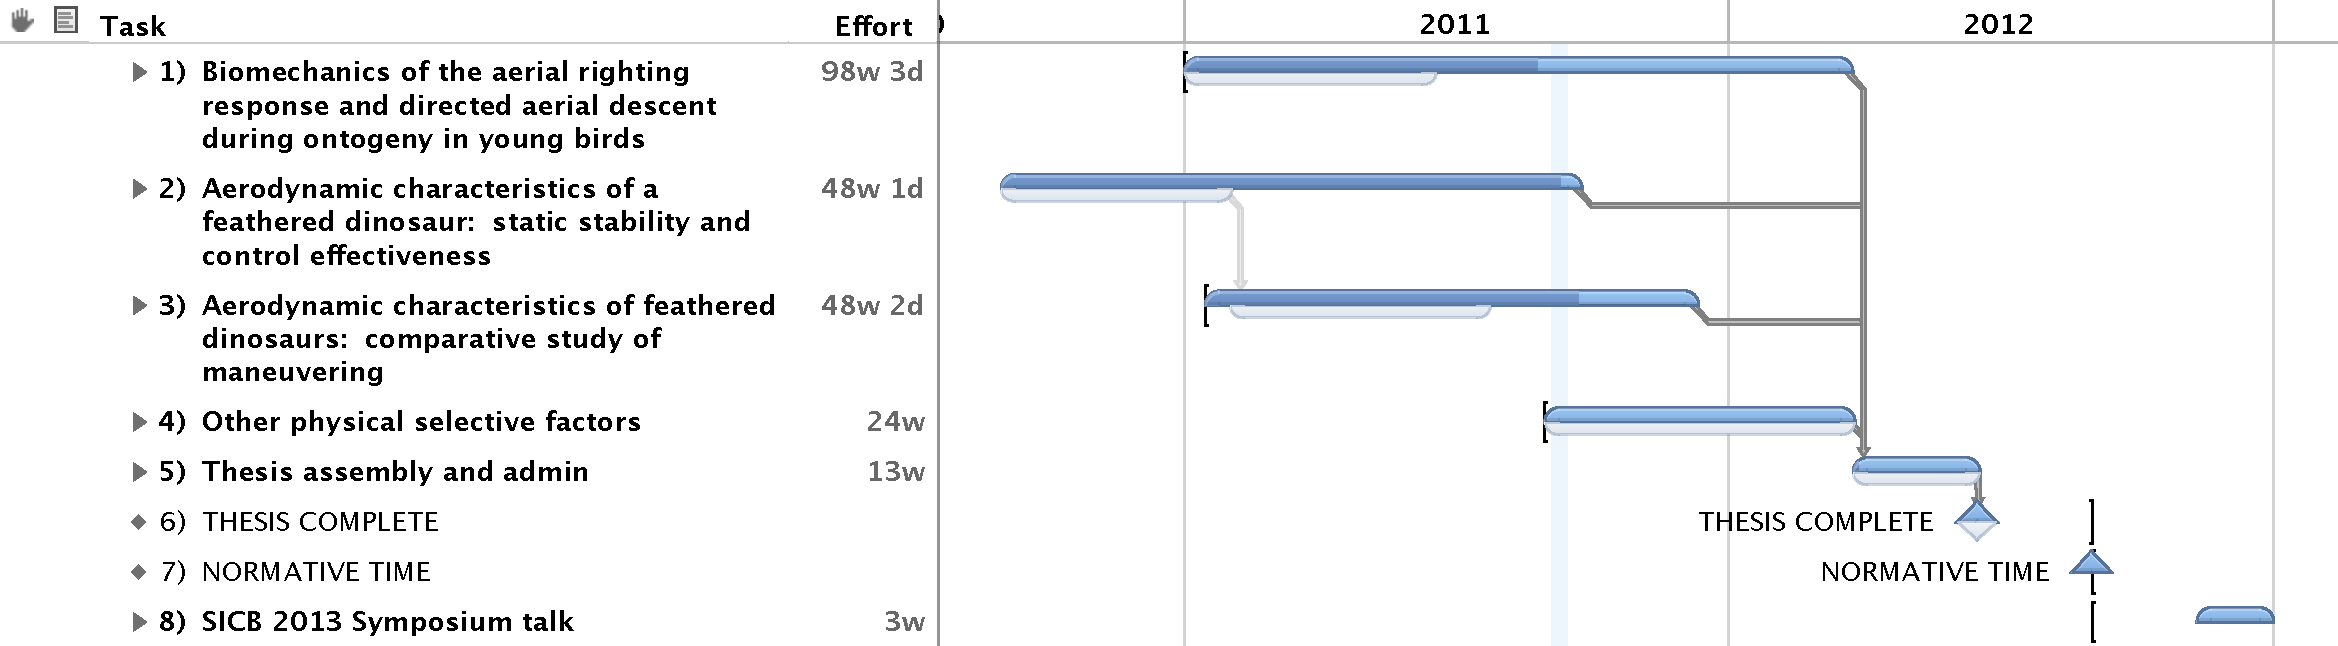
\includegraphics[width=9in]{figures/thesis-schedule-gantt.pdf}
\end{sidewaysfigure}

\rcsid{$Id$}
\rcsid{$Header$}
\rcskwsave{$Author$}
\rcskwsave{$Date$} 
\rcskwsave{$Revision$}

\chapter{Aerial righting and directed aerial descent during ontogeny in young birds}
\label{ch:1}
\index{maneuvering during ontogeny|(}

%\begin{abstract}
Abstract here  
%\end{abstract}

\section{Introduction}
\label{sec:1intro}

Write introduction here. 

%Introduction here\footnote{Target journal is \emph{J exp Biol}?} \citep{Dial:2003, Dial:2008}. The aerial righting reflex allows falling animals to reorient the body dorsoventrally, presumably to initiate gliding or parachuting and subsequent landing without injury using the legs.  
%
%Among vertebrates, aerial righting is likely widespread \citep{Dudley:2007} and others.  Aerial righting is achieved in cats and humans using zero-angular-momentum turns in which the body is twisted in sequence to rotate without external aerodynamic torque \citep{Kane:1969, Frohlich:1970, Liu:1985, Edwards:1986}.  In house geckos, aerial righting is similarly accomplished using torques generated by rapid rotation and nutation of the tail \citep{Jusufi:2008}.  (Fish? Frogs?)  
%
%Among terrestrial arthropods, aerial righting in stick insects (Zeng in preparation) is currently under study, and preliminary work indicates aerodynamic torques is dominates aerial righting (compared to inertial torques) in smaller stages.    
%
%(Has aerial righting been described in extant archosaurs, and have previous aerial righting studies considered size and aerodynamic effects?)  Do young birds possess an aerial righting reflex?  If so, how is aerial righting accomplished, and how does it change during ontogeny? 
%
%Previous workers have used the Chukar Partridge (\Alectorischukar), a ground-dwelling game bird native to Asia but imported to the US, as a model system to explore the use of the wings to assist incline running.  For comparison to this existing data set, chukars are a logical candidate for these experiments.  Alternative study organisms could include chickens or ducks (readily available from agricultural sources and able to be re-homed following experiments) or other birds in families that have evolved flightlessness (Ratites, penguins, kakapo parrots) or compromised flight abilities (various other running galliforms, puffins, cormorants).  However, unfortunately, unlike in stick insects, none of these has reversed the wing loss.  Another possibility is those birds for whom directed aerial descent in chicks is ecologically relevant (tree-nesting birds like murrelets or wood ducks). 

\section{Methods and materials}
\label{sec:1methods}

\subsection{Study animals}
A total of 29 Chukar Partridges (\Alectorischukar) in five batches, $x$ male and $y$ female, aged one day-post-hatching (dph), were obtained by hatching eggs from a local game bird farm (Fall Creek Game Birds; Felton, CA).  Clean, unwashed eggs were placed in a forced air incubator (HovaBator, GQF Manufacturing; Savannah, GA) equipped with a turning tray.  Eggs were held at \SI{37.5}{\celsius} (\SI{99.5}{\SIUnitSymbolDegree F}) for \SI{24}{\day}; turning was discontinued at \SI{21}{\day}.  Upon hatching, chicks were allowed to dry in the incubator for \SI{12}{\hour} and transferred to a brooder bin.  During the course of experiments, chicks were housed in \SI{53x38x30}{\centi\meter} brooder bins heated with two \SI{100}{\watt} floodlamps to maintain a brooder temperature of \SI{29.4}{\celsius} the first week, \SI{26.7}{\celsius} the second, and \SI{23.9}{\celsius} for subsequent weeks.  Birds were kept on wood shavings and offered crumbled chick starter rations (Purina; St.\ Louis, MO) and water \emph{ad libitum}.  Birds were also offered grit, freshly cut grass and mealworms. Chukars were studied at ages between \SIrange{1}{28}{dph}.  All handling of chicks and eggs was under protocols approved by the UC Berkeley Animal Care and Use Committee (ACUC).

To provide comparison with a species with slower wing development, a single batch of five Mallard Ducks (\Anasplatyrhynchos), 2 male and 3 female, was obtained as day-old-hatchlings from a local waterfowl farm (Metzer Farms; Gonzales, CA). Ducklings were housed on absorbent bedding in a large fiberglass tub and were fed on higher-protein waterfowl starter (Mazuri, Somewhere, NC).  Care of ducklings was similar to care for Chukar chicks, using protocols approved by the UC Berkeley ACUC.  Ducks were studied at ages between \SIrange{1}{70}{dph}.

For all birds, weights, lengths, and areas were measured daily to allow computation of wingspan, aspect ratio, area, and wing loading.  Birds were weighed using a digital scale (Scout Pro; Ohaus, Parsipanny, NJ).  Lengths and areas were obtained by restraining birds by hand against a gridded board and photographing using a digital camera (Canon PowerShot SD550); the photos were then digitized using ImageJ (NIH, Bethesda, MD). 

\subsection{Drop tests and manipulations}

Drop tests were conducted using methods similar to \citep{Jusufi:2008, Munk:2011, Zeng:2011}.  Birds were dropped in several different initial orientations (described below), from heights ranging between \SIrange{0.5}{2.5}{\meter}.  Aerial behaviors were captured using a suite of high speed and conventional digital video cameras.  High speed cameras consisted of between one and three cameras (AOS Technologies AG, Baden Daettwil, Switzerland; or Fastec Imaging, San Diego, CA) operated at \SI{500}{frames\per\second}, with one camera filming from the front and additional cameras filming from above or to the side.  Conventional cameras consisted of up to seven high definition (HD) cameras (FlipHD, Cisco Systems, San Francisco, CA), typically with four cameras filming at different angles from the front and additional cameras filming from above or to the side.  Camera pose and focus (intrinsic) parameters were estimated by filming a calibrated calibration object and using a Levenberg-Marquardt algorithm to minimize reprojection error, as described below.  Body positions were then digitized frame by frame using ImageJ (NIH, Bethesda, MD) and the resulting kinematics were analyzed as described below. 

The first batch of Chukars and the first batch of Mallard Ducks were dropped with upright, \ang{90}, and inverted (\ang{180}) orientations presented at random.  It was found that righting from the fully inverted position occurred very quickly in both (Section~\ref{sec:1results}, within \SI{4}{dph}) and that drops from upright position always remained upright.  Accordingly, subsequent drops were conducted only from the inverted position. 

In Chukar, manipulations to augment tail inertia were attempted by attaching plastic prosthetic long tails using veterinary wrap.  Tail augmentation was not successful\footnote{Birds tended to foul the prosthetic tail or mounting vet wrap with feces or groom it off.} and are not reported further here.  Symmetric and asymmetric clipping of wings (all remiges proximal to the outermost secondaries) and complete clipping of the tail (all retrices) were also performed at the end of all other runs.  

\subsection{Two-dimensional analysis}

As a first cut, a two-dimensional (2D) analysis was conducted to identify overall performance and changes during ontogeny.  2D analysis used a single side- or front view high-speed camera calibrated using scales within the image.  From the single view, 
the response time, righting angular velocity and angular position during the maneuver, vertical descent velocity, overall height lost, and success (\%) at righting were obtained. In additional, the righting method (discussed in Section~\ref{sec:1results}) was noted.  These were obtained for all ages.  

\subsection{Three-dimensional analyses}

For selected runs, a three-dimensional analysis was conducted to identify more precisely the onset of aerial behaviors and to determine the role of limb, tail, and body inertia in maneuvers.  

To perform three-dimensional analyses, a camera calibration technique was developed based on \cite{Munk:2011, Bradski:2008}. The calibration made use of homography transforms for multiple views of a two-dimensional chessboard calibration object to obtain camera poses (3D position and rotation), focus (intrinsic) parameters, and relative positions to one another.  With the camera parameters and with homologous points digitized in each image from each camera, a minimization routine was used to minimize the 2D reprojection error of the estimated 3D position. The method differs from \citep{Munk:2011} in the use of homography transforms and a 2D, repositionable calibration object compared to the large and fixed frame of \citep{Munk:2011}; this makes the method here more field-portable and easy to setup.  Details of the method are given in Appendix~\ref{app:cam}.  

The onset of aerial behaviors was detected by examining where the observed behaviors are no long well-described by a passive ballistic null model.  In the absence of any aerial behavior, the path of a falling object can be predicted using ballistics, \emph{i.e.\ } gravity, perhaps with drag.  The onset of aerial behavior is observed when we can detect behavior that deviates from this prediction.  To accomplish this, the likelihood of a given 3D trajectory was computed based on several candidate models for the behavior.  These were then compared using an Akaike Information Criterion (AIC):  
\begin{equation}
\mbox{AIC} = 2 k - 2 \ln(\mathcal{L})
\end{equation}
The candidate models are given by:
\begin{align}
\notag g_0:  x &= X_0 + \mathcal{N}(0,\sigma)& &\text{(stationary)}\\
\notag g_1:  x &= X_0 + V t + \mathcal{N}(0,\sigma)& &\text{(constant velocity)}\\
\notag g_2:  x &= X_0 + V t + \frac{1}{2}a t^2 + \mathcal{N}(0,\sigma)& &\text{(constant acceleration)}\\
\notag g_2':  x &= X_0 + V t - \frac{1}{2} \num{9.81} t^2 + \mathcal{N}(0,\sigma)& &\text{(Earth gravity)}\\
%\notag g_3:  x &= X_0 + V t + \frac{1}{2}a t^2 +\frac{1}{6}b t^3 + \mathcal{N}(0,\sigma)& &\text{(constant jerk)}\\
\notag g_3:  x &= X_0 + V t + X_1 e^{-t/\tau} + \mathcal{N}(0,\sigma)& &\text{(linear drag terminal velocity)}
\end{align}
 The derivation of these methods is given in Appendix~\ref{app:tdd}.

The relative role of inertia in accomplishing maneuvers was examined using a numerical method to predict how the maneuver would unfold in the absence of any aerodynamic forces.  The method is derived in Appendix~\ref{app:ang}.  Point masses are assigned 3D positions based on digitized body and limb positions obtained as described above.  These are then used in a forward calculation, to calculate the angular momentum and examine if it is constant (as would be predicted in a maneuver dominated by inertia) or if it is time-varying (as would be predicted where aerodynamic forces and torques are large).  The same data were also used in a reverse calculation, to obtain the whole body rotation that would result in a solely inertia case (i.e.\ in the case of a bird flying in a vacuum).  The methods here are superficially similar to \citep{Jusufi:2008, Bergou:2011} but avoid the need to derive explicit analytical expressions for multi-axis constrained linkages.  By numerically performing this calculation, this method is more applicable to a wider range of geometries and situations where the inertia acting to accomplish the maneuver is not straightforward to identify and lump into a single rotating element. 



\section{Results}
\label{sec:1results}
Write results here. 

\subsection{Morphometrics}
Figure~\ref{fig:1mass} shows chukar mass as a function of age.  
%Are there individual effects, yes probably.  Are there sex differences, I'm not sure. So maybe I'll have to plot the aerodynamic results versus mass, rather than age in days-post-hatching (doh), and will have to similarly convert the Dial stuff? 

\begin{figure}
\begin{center}
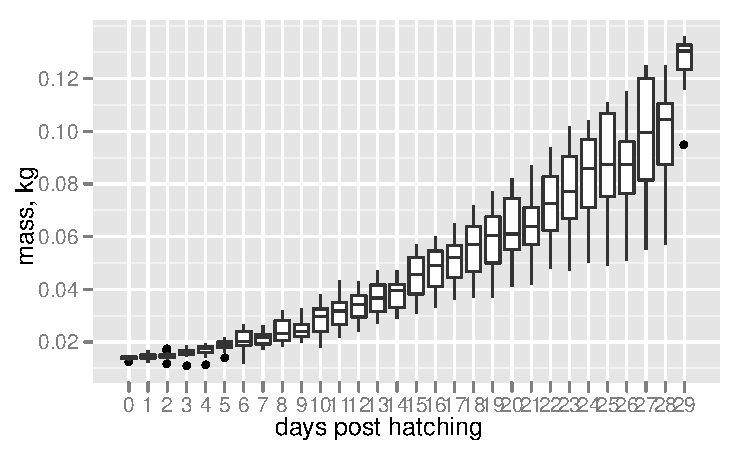
\includegraphics{figures/chukar-mass-boxplot.pdf}
\end{center}
\caption{Boxplot of chukar mass versus age. Explain what symbols are. Might be good to turn x-axis labels to avoid crowding.}
\label{fig:1mass}
\end{figure}

\subsection{Overall descent metrics}
\subsection{Onset of directed aerial descent}
\subsection{Inertial contribution to turns}


\section{Discussion}
\label{sec:1discussion}
Write discussion here. 

%\subsection{Evolutionary significance for the origins of bird flight}
%Birds lack a massive tail (unlike geckos) and their axial skeleton is stiffened by imbricated ribs and by the widespread fusion at the synsacrum (unlike mammals).  I would expect the avenues available to other vertebrate taxa for generating zero-angular-momentum turns are not present in birds, and dynamic models based on these other taxa should fail to predict the observed kinematics unless aerodynamic terms related to the wings or legs are added.  To test this further, patches could be used to augment areas (to simulate plumage changes with size held constant).  
%
%Theropod ancestors of birds had similar hips but lacked the rib cage stiffening; they also possessed long tails, and studies of falling bird chicks alone may not fully address this.  I may wish to test this further by manipulations to increase tail inertia by adding a boom similar to a theropod tail, or by testing aerial righting reflexes in other archosaurs (caimans).  This would provide a (somewhat weak) extant phylogenetic bracket for the presence of aerial righting in bird ancestors.
%
%The size-scaling of aerial righting ability may also be informative.  Many phylogenetic reconstructions of size in the clades leading to birds suggest they were small, perhaps small enough that both inertia and aerodynamics are important in the initial aerial righting given the phylogenetic constraints on axial body movement.  


\section{Acknowledgements}
We thank Dylan Marks for his assistance with filming.  We thank Luis Guillen and Kathy Moorhouse for their advice and assistance in raising birds.  We thank the Berkeley Center for Integrative Biomechanics Education and Research for the use of high speed cameras.  We thank Lindsay Waldrop, Kelly Dorgan, Yonatan Munk, Yu Zeng, Erica Kim, Marc Badger, Sofia Chang, Nir Sapir, Victor Ortega, and Marta Wolf for their analysis suggestions, assistance and support.  DE was supported by an NSF IGERT Fellowship and by a grant from the National and Berkeley local chapter of Sigma Xi.

\index{maneuvering during ontogeny|)}

% \bibliography{references/chukar} % copy all citations from this to main bibliography




\appendix
\rcsid{$Id$}
\rcsid{$Header$}
\rcskwsave{$Author$}
\rcskwsave{$Date$} 
\rcskwsave{$Revision$}

\chapter{\emph{Alectoris chukar} Animal Use Protocol}
\label{app:AUP}
\index{Chukar}
\index{Alectoris chukar@\textit{Alectoris chukar}}
\index{Animal Use Protocol|(}
The following are excerpts from UC Berkeley Animal Use Protocol R282, revision 1 for the use of Chukars (\emph{Alectoris chukar}) in studies of directed aerial descent and righting.

\section{Research goals}
\index{Animal Use Protocol!goals}
Existing paleobiological scenarios for the origin of flapping flight in bats, birds, and pterosaurs strongly implicate transition from a gliding and maneuvering form, but the biomechanical and aerodynamic correlates of this transition are unclear. To examine biomechanical constraints relevant to such a transition, recent and past work includes studies of falling geckos \citep{Jusufi:2008}, gliding frogs \citep{Emerson:1990, McCay:2001}, extinct feathered dinosaurs \citep{Xing:2003}, and flying squirrels.  Other parallel work in invertebrate taxa, such as gliding ants \citep{Yanoviak:2005} and gliding stick insects also strongly implicate transition from a gliding and maneuvering form.

An alternate scenario for the origin of flapping flight in vertebrates involves the use of wings to assist running and traction up steep terrain \citetext{wing-assisted incline running, \citealp{Dial:2003, Bundle:2003, Dial:2008}}.  Studies in support of this alternative scenario have observed that hatchling birds utilize flapping movements when running up inclines \citep{Dial:2008}.   However, these studies ignore use of the wings during other aerial-related behaviors, for example, use of the wings when descending vertically.  Using the same species and general experimental setup, we plan to address this gap by determining limb and body kinematics, both symmetric and asymmetric, that contribute to aerial righting and directed aerial descent maneuvers, and that may have historically led to bilateral limb flapping in birds.  Wind tunnel studies of static and flapping models and computer simulations based on aerodynamics and inertial mechanics will complement these kinematic studies.


\section{Justification for animal use}
\index{Animal Use Protocol!justification for animal use}
\subsection{Rationale for use of animals}
Flying and gliding animals are paradigmatic examples of the generation and control of unsteady aerodynamic forces, and exhibit both neuromuscular regulation and multimodal sensory integration that far surpass current technological capacities.  To understand both generation and control of these aerodynamic phenomena, it is necessary to study living animals as they naturally locomote in the air.

\subsection{Rationale for choice of species and numbers}
Chukar Partridges are a model system for wing-assisted inclined running; as this work examines a gap in WAIR theory and seeks to extend it, they are a logical choice to start with as the data obtained will be directly comparable to previous studies \citep{Bundle:2003, Dial:2003, Dial:2008}.  Chukars are widely available through the poultry trade \citep{Heinrichs:2009, OToole:2003, Willis:2009}.  The number of study birds is based on our lab�s previous work in similar kinematic studies and should provide sufficient replicate measurements. \index{Animal Use Protocol!species rationale}\index{Animal Use Protocol!number rationale}


\section{Description of laboratory research}
\index{Animal Use Protocol!research description}
With Chukar Partridges, we seek to determine 1) the presence or absence of an aerial righting reflex over ontogeny; 2) the presence or absence of directed aerial descent ability over ontogeny; 3) three-dimensional trajectories and limb and tail usage during such maneuvers; and 4) the impact of a limited set of non-invasive manipulations (attachment/augmentation of feathers, especially pelvic wing feathers \citep{Lippincott:1920, Xing:2003, Thomas:1997, Evans:1992, Evans:1994} and augmentation of tail inertia \citep{Jusufi:2008}.  

All experiments will involve filming with video cameras illuminated with \SI{500}{\watt} lights.  Each filming event lasts up to thirty seconds.  Birds may be filmed on a daily basis for periods of three hours  During all experiments, animals will be observed for signs of weakness and will be removed from the study if such signs are evident.  Animals showing signs of reluctance will be given time to habituate to experimental setups.  Animals may be non-destructively marked by either attachment of adhesive-backed \SI{3}{\milli\meter} reflectors  or use of Wite-out and black marker, both typical in other studies of bird locomotion \citep{Dial:2008, Hedrick:2007, Daley:2007, Essner:2002, Wischusen:1989}.  During marking, animals will be restrained by hand.


\subsection{Presence or absence of aerial righting reflexes over ontogeny}
Chicks will be placed on a platform such as a ladder and allowed to take off freely, or dropped at a random orientation by tipping out of a cup.  Their vertical orientation will be observed during descent using high-speed video recording of kinematics.  Gentle vibration may be applied to the cup to induce takeoff.  The experimental setup will provide for a soft landing area, such as a loosely spanned, soft and eleastic cloth or foam.  The methods here will be identical to those we have used to study aerial righting and directed aerial descent in rain forest canopy ants, stick insects, and also in geckos \citep{Jusufi:2008}.\index{Animal Use Protocol!kinematics}

All chukar experiments will be conducted using a ladder, ramp, or scaffold structure within a \SI{5 x 3}{\meter} full-ceiling-height animal enclosure with fabric or netting walls in Haas 97/99.  For runs in which voluntary bird behavior is recorded, filming will be conducted up to daily for up to three hours per day.  For runs in which birds are gently stimulated, \SI{5}{\minute} rest periods will be provided between glides and a \SI{30}{\minute} rest every five glides, with an absolute maximum of 15 glides per animal per day. \index{Animal Use Protocol! drop tests} 

\subsection{Presence or absence of directed aerial descent ability over ontogeny}
Using methods similar to \citep{Dial:2008}, chicks will be allowed to run up an incline and jump off it freely; or will be placed at the top of an obstacle and gently stimulated to descend from it into a soft landing area. Filming of the descent with multiple high-speed video cameras will assess if trajectories show evidence of turns or if they are random or confined to a single plane \citep{Essner:2002, Socha:2002}.  Most runs will film the free, volitional behavior of chicks as they explore the experimental setup.  

To provide additional testing of the extent of directed aerial descent abilities, the target landing zone may be displaced over small distances after the chick jumps, as has been done in what was done in previous studies of flying squirrels \citep{Wischusen:1990}.

\subsection{Three-dimensional trajectories and limb and tail usage during such maneuvers}
Part of this experiment will be conducted concurrently with experiments 1 and 2, which already film the animals using multiple high-speed video cameras that are sufficient to obtain three-dimensional trajectories and appendage use during maneuvers.  

To obtain additional information on aerodynamic use of appendages , chicks may be placed in the working section of a vertical wind tunnel  to simulate conditions of free fall \citep{McCay:2001, Jusufi:2008}. Equilibrium gliding at terminal falling velocity is reached when the aerodynamic drag and lift forces balance the force of gravity. A small animal like a Chukar Partridge will attain terminal velocity at a ventral airflow of less than \SI{6}{\meter\per\second}, depending on individual mass and surface area.  Chicks will not be exposed to air speeds exceeding the equivalent of individual terminal velocity. To prevent chicks from maneuvering sideways out of the test section and to enable high-speed video filming, transparent acrylic sidewalls will be mounted around the opening of the wind tunnel. A safety net will be installed in the test section to prevent animals from contacting the expansion chamber of the wind tunnel.\index{Animal Use Protocol! use of wind tunnel}


\subsection{Relative effects of inertia and aerodynamic forces in maneuvers}
 To examine the role of inertia, small weights no more than \SI{10}{\percent} of body weight will be attached to the chicks using veterinary wrap, similar to methods used in \citep{Daley:2007}.  Inertia will be increased by addition of a ``prosthetic tail'' made from a lightweight shaft (e.g. music wire, wood, plastic or cut turkey feathers) with a small weight held onto to the chick�s natural tail using veterinary wrap.  For control purposes, an equivalent amount of weight may be added at the hips, near the center of mass, or on a leg or wing \citetext{as in \citealp{Daley:2007}}. Weights will be removed at the end of each session. index{Animal Use Protocol!inertial augmentation}
 
To examine the role of aerodynamic forces, we will observe aerial behaviors over ontogeny as the bird�s natural feathers develop.  In addition, we may clip the primary feathers and retrices, augment the primary feathers or retrices by gluing of additional feather extensions \citetext{\citealp{Evans:1994}, approved UCB Animal Use Protocol R282}, or augment feathers by gluing flight feathers at the position of other, non-flight feathers such as the pelvic ``wing'' plumage \citep{Lippincott:1920}.
 
Feather extensions will be conducted using the method of \citet{Evans:1994}.  Feathers will be cut near the base and new feathers glued on to vary length from between \SIrange{5}{10}{\percent} of the original length.  Feather extensions will be glued using a combination of pins and cyanoacrylate superglue.  Attached feathers will have been frozen several months to kill any parasites that may have been present. 
During these manipulations, chicks will be restrained by hand.  No anesthetization is necessary because the manipulations involve no living tissue; no living tissue is manipulated other than whole-body restraint for no more than \SI{10}{\minute} during these procedures.  Feathers are attached carefully so that they retain aerodynamic function; this method has been used extensively for other avian taxa \citep{Evans:1994, Evans:1992, Thomas:1997} and these authors report that manipulated birds folded their tails naturally and did not pick at or seem to unduly notice the manipulated feathers.  Maneuverability and aerodynamic performance of individuals with manipulations will be assessed using the methods described above.  Upon completion of manipulation experiments, manipulated feathers will be plucked to induce their replacement.  Birds that pick at extensions will have the extensions checked and adjusted as practicable and will be given time to acclimate, but extensive picking or grooming of the extensions may invalidate the experiment and such birds will be removed from study. \index{Animal Use Protocol!feather extensions}

\section{Method of euthanasia and disposition of specimens}
\index{Animal Use Protocol!euthanasia}
Euthanasia, if needed for Chukar Partridges at study's completion: overdose of isoflurane or carbon dioxide inhalation followed by bilateral thoracotomy.

\section{Proposed animal housing}
Chukar Partridges will be maintained within the Animal Behavior Research Suites on the fifth floor of VLSB.  Chukar Partridge chicks will be maintained within the Animal Behavior Research Suites on the fifth floor of VLSB.  Birds will be kept on brooder bedding litter (wood shavings, sawdust, compressed wood pellets, or other suitable material) changed bi-weekly or as necessary \citep{Heinrichs:2009, Willis:2009}.  Lamps will be provided to maintain a warm temperature as necessary \citep{Heinrichs:2009, Willis:2009}.  Birds will be kept in an enclosure with approximately 25 chicks to a \num{4 x 3} foot area \citep{Heinrichs:2009, Willis:2009}.  We will keep an individual Chukar Partridge for up to eight weeks, to allow completion study up to the point of being fully feathered and slightly beyond.  Most work will be completed at approximately four weeks.  Batches of chicks will not be mixed and additional space will be provided as birds age beyond four weeks (approximately \num{2} square feet per bird) \citep{Heinrichs:2009, Willis:2009}. \index{Animal Use Protocol!housing}

Chukar Partridge will be fed typical chick starter rations (\SI{20}{\percent} protein) in suitably designed feeding containers \citep{Heinrichs:2009, Willis:2009}.  OLAC personnel will feed the birds daily following standard UCB arrangements.  Diet will occasionally be supplemented with grit, vegetable material, or insect larvae \citep{Heinrichs:2009, Willis:2009}.  Water will be available at all times in suitably designed watering containers no more than a few inches deep \citep{Heinrichs:2009, Willis:2009}. \index{Animal Use Protocol!feeding}

When Chukar Partridges are returned to fifth floor housing after flight experiments, they will be monitored one hour after return and again the following morning to ensure normal behavior.  We typically check in on all of our animals one to two times daily independent of the occurrence of flight experiments.
	
\section{Breeding}
No breeding will be undertaken. \index{Animal Use Protocol!breeding}

\section{Capture and transportation of animals}
Chukar Partridges will be obtained as one-day-old chicks and shipped via standard shipping methods for poultry \citep{Heinrichs:2009, Willis:2009}.   For experiments, chicks will be transported between the Animal Behavior Research Suites on the fifth floor of VLSB and Haas 97/99 (a one minute walk) using a small animal carrier with litter and provision for ventilation.  No more than 12 chicks will be placed in one box (or less depending on size).  \index{Animal Use Protocol!transport of birds}

\section{Description of field research}
No field components are associated with studies of Chukar Partridges.\index{Animal Use Protocol!field research}

\index{Animal Use Protocol|)}


\rcsid{$Id$}
\rcsid{$Header$}
\rcskwsave{$Author$}
\rcskwsave{$Date$} 
\rcskwsave{$Revision$}

\chapter{Camera calibration and three-dimensional reconstruction routine}
\label{app:cam}
\index{camera calibration|(}

This appendix describes a method to recover the three-dimensional (3D) position of birds and their appendages using several two-dimensional (2D) views, obtained from cheap fixed-focus FlipHD cameras.  The methods are also applicable to AOS and Fastec high speed cameras used in other parts of the work.  

While the techniques are similar to those used to track ants in the rain forest \cite{Munk:2011}, and to methods I used to track ballistically launched amphipods (cite me), there are some important differences incorporated here in order to make simplify the calibration procedure and setup. The primary difference is the use of multiple views of multiple poses of a two dimensional calibration object (chessboard), enabled by use of homographies, freeing the setup from the need for a large, fixed calibration shape that remains present and un-moved/un-altered through all filming runs.  This reduces setup time and is critical when cameras must be shared between multiple setups and must be setup and broken down each day or multiple times each day.  

% needed in second column of first page if using \IEEEpubid
%\IEEEpubidadjcol


\section{Camera extrinsics}
In computer vision applications, it is typical to convert from world coordinates to camera-fixed spatial coordinates using a translation $\vec{t}$, followed by rotations about $\hat{z}$, then the new $\hat{y}$, then the new $\hat{x}$ (in that order) \cite{Bradski:2008}. 
\begin{equation}
\mathbf{R_x}(\psi) =
\begin{pmatrix}
1 & 0 & 0 \\ 0 & \cos{\psi} & \sin{\psi} \\ 0 & -\sin{\psi} & \cos{\psi}
\end{pmatrix}
\end{equation}
\begin{equation}
\mathbf{R_y}(\phi) =
\begin{pmatrix}
\cos{\phi} & 0 & -\sin{\phi} \\
0 & 1 & 0 \\
\sin{\phi} & 0 & \cos{\phi}
\end{pmatrix}
\end{equation}
\begin{equation}
\mathbf{R_z}(\theta) = 
\begin{pmatrix}
\cos{\theta} & \sin{\theta} & 0 \\
-\sin{\theta} & \cos{\theta} & 0 \\
0 & 0 & 1
\end{pmatrix}
\end{equation}
\begin{equation}
\vec{x}_{cam} = 
\mathbf{R_x R_y R_z}
(\vec{x}_{world} - \vec{t})
\end{equation}
\begin{equation}
\vec{x}_{cam} = 
\mathbf{R}
(\vec{x}_{world} - \vec{t})
\end{equation}
The inverse of this operation is given by:
\begin{equation}
\vec{x}_{world}
=
\mathbf{R}^{-1} \vec{x}_{cam} + \vec{t} 
\end{equation}
where
\begin{equation}
\mathbf{R}^{-1} =
\mathbf{R}^T =
\mathbf{R_z}^T \mathbf{R_y}^T
\mathbf{R_x}^T
\end{equation}
Alternatives to this formulation include axis-angle and quaternion methods, which avoid problems at \ang{+-90} pitch angles.  This is often handy, e.g. when integrating inertial sensor data, but for now we will stick to the orthogonal rotation matrix method as it is standard in computer graphics practice. 

\section{Camera intrinsics and pinhole model}
It is useful at this point to introduce homogenous coordinates, in which a point in an $n$-dimensional space is expressed as an $n+1$-dimensional vector; any two points whose values are proportional (``within a scale factor'') are equivalent \cite{Bradski:2008}.  The pinhole model of camera is thus: 
\begin{equation}
\begin{pmatrix}
x \\ y \\ w
\end{pmatrix}_{im}
=
\begin{pmatrix}
f_x & 0 & c_x \\
0 & f_y & c_y \\
0 & 0 & 1
\end{pmatrix}
\begin{pmatrix}
x \\ y \\ z
\end{pmatrix}_{cam}
\end{equation}
where $f$ is the focal length and $c$ is the displacement of the imaging plane from optical zero.  To find pixel coordinates we make use of the equivalence of homogenous coordinates, i.e. $x_{pal} = x_{im}/w_{im}$ and $y_{pel} = y_{im}/w_{im}$.

\section{Homography, chessboards, and calibration}
Ignoring distortion, we can map real world coordinates to image coordinates using the following:
\begin{equation}
\begin{pmatrix}
x \\ y \\ 1
\end{pmatrix}_{im}
=
s
\begin{pmatrix}
f_x & 0 & c_x \\
0 & f_y & c_y \\
0 & 0 & 1
\end{pmatrix}
\begin{pmatrix}
\vdots & \vdots & \vdots & \vdots \\
\vec{r}_1    & \vec{r}_2    & \vec{r}_3    & \vec{t} \\
\vdots & \vdots & \vdots & \vdots
\end{pmatrix}
\begin{pmatrix}
x \\ y \\ z \\ 1
\end{pmatrix}_{world}
\end{equation}
Rearranging for the case of a flat chessboard on which we arbitrarily pick $z=0$,
\begin{equation}
\begin{pmatrix}
x \\ y \\ 1
\end{pmatrix}_{im}
=
s
\begin{pmatrix}
f_x & 0 & c_x \\
0 & f_y & c_y \\
0 & 0 & 1
\end{pmatrix}
\begin{pmatrix}
\vdots & \vdots & \vdots \\
\vec{r}_1 & \vec{r}_2 & \vec{t} \\
\vdots & \vdots & \vdots
\end{pmatrix}
\begin{pmatrix}
x \\ y \\ 1
\end{pmatrix}_{chessboard}
\end{equation}
Collecting the matrices into a single homography matrix for a particular view (source and destination pair) gives:
\begin{equation}
\vec{p}_{dest} = \mathbf{H} \vec{p}_{source}
\end{equation}
By collecting many points in a particular view, a best-fit $\mathbf{\hat{H}}$ can be found that minimizes the back projection error $\sum \|\vec{p}_{dest}-\mathbf{\hat{H}}\vec{p}_{source} \|$. Open source camera calibration routines then use numerically determined $\mathbf{\hat{H}}$ for many views, and the constraints of orthonormality to obtain camera intrinsics, as well as extrinsic parameters for each particular view \cite{Bradski:2008}.  

\section{Correcting for distortion}
Distortion from cheap lenses and short focal lengths is expected to be large.  It is possible to run the calibration ignoring distortion, then solve for distortion parameters and iterate until convergence \cite{Bradski:2008}. Radial distortion arises from the lens and is given by:
\begin{equation}
x_{corr} = x (1+k_1 r^2 + k_2 r^4 + k_3 r^6)
\end{equation}
\begin{equation}
y_{corr} = y (1+k_1 r^2 + k_2 r^4 + k_3 r^6)
\end{equation}
Tangential distortion arises from skewed mounting of the sensor and is given by: 
\begin{equation}
x_{corr} = x + [2 p_1 y + p_2 (r^2 + 2 x^2)]
\end{equation}
\begin{equation}
y_{corr} = y + [p_1 (r^2 + 2 y^2) + 2 p_2 x]
\end{equation}

\section{Completing the calibration}
The equations given so far are combined in the OpenCV routine \texttt{cvCalibrateCamera2()}, which allows solving for a single camera's intrinsic and distortion parameters and the extrinsic rotation and translation associated with each view used.  The next step is to combine information from multiple cameras.  While most computer vision texts focus on stereo vision applications and use of epipolar geometry and fundamental matrices \cite{Bradski:2008}, we are more concerned with more than two cameras, in arbitrary arrangements that make such approaches non-intuitive.  The stereo vision application is also optimized somewhat for speed (by reducing search dimensionality using epipolars); while here we wish to search in 3D and find the most accurate positions possible. 

From the single camera calibration, we have an initial guess of the position of the cameras relative to one another.  However, we have a lot of extra parameters since the calibration shape is the same in all views.  The next step is to re-run the calibration with some of these extra parameters fixed.  How the heck do we do that? We sort of have to break into the calibration routine and recast the objective function... I suppose I could run pairwise stereo calibrations with the zero camera. 

\section{Locating points}
Once we have the calibrations, we take the approach of \cite{Munk:2011} to find 3D positions from multiple 2D images.  To accomplish this, we assume a position and minimize the squared projection error in all images:
\begin{equation}
\hat{x}_{world} = 
\argmin V
\end{equation}
\begin{equation}
V =
\sum_{all\ cameras} 
\| \vec{x} - s \mathbf{M} 
\begin{bmatrix}
\mathbf{R} & \vec{t}
\end{bmatrix}
\hat{x}_{world}
\|
\end{equation}
where $s$, $\mathbf{M}$, $\mathbf{R}$, and $\vec{t}$ were all obtained from the calibration step. 


% use section* for acknowledgement
\section*{Acknowledgment}
I thank Yonatan Munk for his assistance in implementing these improved methods.  I also thank the Berkeley Center for Integrative Biomechanics Education and Research (CIBER) for providing camera availability problems that motivated this work.  

\index{camera calibration|)}


\rcsid{$Id$}
\rcsid{$Header$}
\rcskwsave{$Author$}
\rcskwsave{$Date$} 
\rcskwsave{$Revision$}

\chapter{Testing for directed aerial descent using an Akaike Information Criterion}
\label{app:tdd}
\index{trajectory testing|(}

These notes give my thoughts on how to test a recorded animal trajectory for directed aerial descent using log-likelihood functions and the Akaike Information Criterion (AIC).\footnote{Several undergraduates helped me to crystallize some of these thoughts when we were puzzling over how, using finite differences, some animals dropped from a ladder in Haas gymnasium, could reach accelerations of \SI[separate-uncertainty]{+-900}{\meter\per\second\squared}; Dave Bapst assured me I was not on crack.}

\section{Introduction}
In studies of the comparative biomechanics of aerial behaviors, we often obtain the trajectory of an animal traveling through space and we wish to decide if it is moving as a passive ballistic projectile would, or if it is ``doing something.'' Is it using bits of its body to generate forces and moments that change its trajectory through the air in order to right itself, land on some target, move towards some goal or away from something it wishes to avoid?  More generally, we wish to test some data and see if it is well explained by a certain model with some terms, or if an alternative model with other terms is a better description.  We may also need (or have) some idea of what our measurement noise is. 

\section{A toy example: estimating position of a stationary object with noisy measurements}
Let us imagine we have a calibrated high speed video recording of a dead limpet on a rock.  Frame by frame, we digitize the $x$ position of the limpet for the portion of the video we wish to analyze.  The data are given in Figure~\ref{fig:limpet}.  While digitizing such positions are tedious, they allow us to answer two questions.  First, what is the position of the limpet?  Second, is it still moving or is it dead?  

To answer the first question, a simple-minded thing to do first would be to simply take the mean of the measured positions.  We could report then the position as the mean along with the standard deviation; the limpet is at \SI[separate-uncertainty]{0.423+-0.001}{\meter}.  This frequentist approach is pretty standard in biology and biomechanics.  

However, we run into problems if we try to answer the second question - is the limpet still moving?  Now we must somehow approximate the derivative.  We may try using a finite difference approximation, approximating the derivative $\frac{dx}{dt}$ as $\frac{x_{n+1}-x_{n}}{\Delta t}$, then testing to see if this is significantly different from zero using an appropriately chosen frequentist statistical test.  The drawback with this is that numerical differentiation in this manner introduces noise, and since we are often after accelerations and forces, which require a second derivative, the noise can quickly mask anything interesting that may be happening in realistic data.  We could employ filters (e.g. Butterworth, Chebyshev, moving average) or interpolating spline procedures, however, these add additional layers of manipulation to the data and may be unintuitive to those not used to filtering approaches.  Furthermore, they do not make use of whatever we might happen to know about the noise in our measuring system. 

\section{An alternative using maximum likelihood estimation}
Let us proceed by imagining a model of the process of measuring the position of a dead, stationary limpet.  Unless it is being moved by something, the limpet's measured position at some discrete time $n$ may be thought of as an actual position plus some additive measurement error:
\begin{equation}
x[n] = X_0 + \mathcal{N}(0,\sigma)
\end{equation}
We might consider this model as a null model for a dead limpet.  $\mathcal{N}$ here is some model of the measurement noise; in this case for simplicity we will consider zero-mean, stationary, Gaussian noise.  For this case, it is clear that our earlier procedure of simply taking the mean and standard deviation of our measurements should recover $X_0$ as the position fo the limpet and $\sigma$ as the standard deviation, provided we take enough samples. 

Let's consider a different approach known as maximum likelihood estimation \cite{Burnham:2002, Rauch:1965}. Imagine we knew $X_0$ and $\sigma$; then we could figure out how likely it is that we observe the actual measurements by computing $P(\text{data}|\text{model},\text{parameters})$:  
\begin{equation}
\ln(\mathcal{L}(X_0,\sigma | x, \text{stationary})) = \sum_n \ln \left(f_{\mathcal{N}(0,\sigma)}(x[n]-X_0) \right)
\end{equation}
$\ln(\mathcal{L})$ is the log-likelihood; it is easier for us to use because it turns the product of many small numbers into a sum of something that is more easily represented within the computational range of our computer.  To figure out the most likely estimate of the position of the limpet (and the noise of our measuring setup), we can search for the values of those parameters that maximize the likelihood:
\begin{equation}
\hat{X_0}, \hat\sigma = \argmin_{X_0, \sigma} \left[ - \sum_n \ln \left(f_{\mathcal{N}(0,\sigma)}(x[n]-X_0) \right) \right]
\label{eq:MLE}
\end{equation}
The search is done in our computer, using whatever minimum-seeking routine we wish to use, such as various flavors of \texttt{fmin} in Matlab, Octave or Python, ``GoalSeek'' in ExcelSucks, etc.  

At first glance, the log-likelihood approach appears to make life more complicated, but it is an improvement.  With our old approach, we heavily manipulate the data to get velocities and accelerations, compute some test statistics (mean, standard deviation) and then perform some set, voodoo-like procedure (ANOVA or non-parametric test) to see if this is different from the position of another dead limpet.  The test procedure is, to many biomechanics practitioners, a black box relegated to a stats course taken long ago.  The old approach is ``no thought required'' - which is precisely its drawback.  By instead modeling the process that produced the measurements, we can get a handle on both the physical process driving the measurement and the measurement noise.  We can also then compare different models, to select which is a more appropriate description of what we have observed.

\section{Comparing models}
Back to the question of is the limpet moving?  Our null approximating model (repeated below) was that it is stationary: 
\begin{equation}
g_0:  x[n] = X_0 + \mathcal{N}(0,\sigma)
\label{eq:stationary}
\end{equation}

A reasonable alternative approximating model is that the limpet is crawling along with some constant velocity $V$:
\begin{equation}
g_1:  x_v[n] = X_0 + V \frac{n}{f} + \mathcal{N}(0,\sigma)
\label{eq:constantv}
\end{equation}
where the positions are sampled at some known sample rate $f$; this is simply $x=X_0+Vt$.  We could perform a log-likelihood calculation for $g_1$ and get a decent guess for what $X_0$, $V$ and $\sigma$ are for that model, noting that we've added an additional parameter $V$.  We might like to know if the data are better explained by $g_0$ or $g_1$? Additionally, if $g_1$ is ``better'', is it better by enough to justify the additional parameter $V$, or are we guilty of what is known as \emph{over fitting}?

\subsection{Akaike information criterion (AIC)}
The Akaike information criterion (AIC) \cite{Akaike:1974} provides a way to compare several candidate approximating models and ask if the additional explanatory power of a given model is worth the extra parameters ($k$ is the number of parameters):  
\begin{equation}
\mbox{AIC} = 2 k - 2 \ln(\mathcal{L})
\end{equation}
The AIC is computed for the maximum likelihood parameter estimate for each model.  The model that best explains the data is the one with the minimum AIC value.  In essence, we are searching for the model that requires as little information as necessary to describe the observed data well.  

We can see that increasing the number of parameters increases the AIC. On the other hand, a model that is more likely to explain the observed data will have a smaller AIC.  Models within 1-2 of the minimum have substantial support and should not be discarded; models within 4-7 have less support and models 10 and above have no support and can be discarded \cite{Akaike:1974, Burnham:2002}.  

%There are alternatives to this procedure; a likelihood ratio test could be used, or an equivalent Bayesian approach adopted.  I am not able enough in probability and statistics to make sense of these yet and the AIC appears to fit my needs.  

%PARAPHRASE- Akaike weights are can be used in model averaging. They represent the relative likelihood of a model. To calculate them, for each model first calculate the relative likelihood of the model, which is just exp( -0.5 * �AIC score for that model). The Akaike weight for a model is this value divided by the sum of these values across all models.
%
%DAVE BAPST NOTES - I'd use AIC weights rather than change in AIC. AIC weights are more easily interpretable for assessing model support. Check Burnham and Anderson for the equation. Gene Hunt has a nice akaike.wts() function in R in his paleoTS library. I'm pretty certain you can do the same thing with the BIC.
%
%DAVE BAPST NOTES - Likelihood ratio tests can only be used if two models are nested, which I think may be the case here (does setting V=0 collapse one model into the other? I think it does.) They are considered 'better' than AIC or BIC (by some people), but you can only compare pairs of models with them and they must be nested. Bayesian analyses are nice in some ways, but its unclear to me why you would want to go that route here. The likelihood method is just simpler and more understandable to non-statistically minded people. If you aren't going to use LRT or Bayesian analysis, I would just drop any mention of those methods.

\subsection{Bayesian information criterion (BIC)}
An alternative to AIC is the Bayesian information criterion (BIC) \cite{Schwarz:1978}.  It is similar in form but includes a term related to the number of observations $n$.  This means that the penalty for having more parameters is larger than in the AIC.  We can check both and see if similar answers are given with each index.
\begin{equation}
\mbox{BIC} = k \ln(n) - 2 \ln(\mathcal{L}) 
\end{equation}



\subsection{So is the limpet moving?}
Let us apply these to some (simulated) limpet data for two limpets, shown in Figure~\ref{fig:limpet}:
\begin{figure}
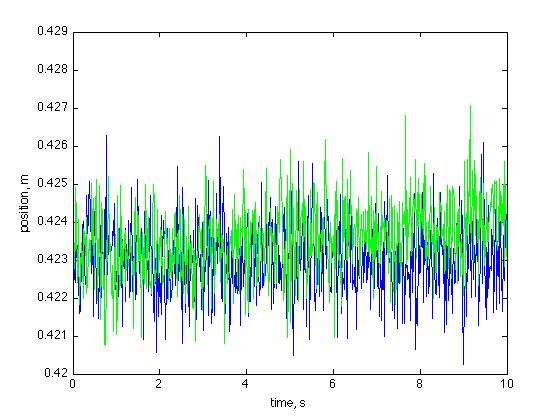
\includegraphics[width=\textwidth]{figures/tdd-Limpet2.jpg}
\caption{Simulated limpet data. Limpet 1 is blue, Limpet 2 is green.}
\label{fig:limpet}
\end{figure}
The simple estimate of the position of Limpet 1 is \SI[separate-uncertainty]{0.423+-0.001}{\meter}, obtained by taking the mean and standard deviation.  If we apply the maximum likelihood estimation algorithm of Equation~\ref{eq:MLE} to Limpet 1, we obtain the same, \SI[separate-uncertainty]{0.423+-0.001}{\meter}.  It's nice to get the right answer (these correspond to the ``true'' values for Limpet 1 in the simulation), and we can go a little further.

We wish to test if the limpets are moving, by checking which fits the data best, stationary model $g_0$, or constant velocity model $g_1$.  Tables~\ref{tbl:limpet} and \ref{tbl:limpet2} summarize the maximum likelihood estimates for the limpets for each model.  The table also contains the AIC and BIC values for the models.  Limpet 1 is stationary and the model with a constant velocity term estimates zero speed (Table~\ref{tbl:limpet}).  We conclude that Limpet 1 is not moving.  On the other hand, there is substantial support that Limpet 2 is moving to the right (Table~\ref{tbl:limpet2}, $\Delta_i\;\text{AIC} = \num{61.1}$).  Comparing the $\Delta_i\;\text{AIC}$ and $\Delta_i\;\text{BIC}$ shows that the constant velocity model has substantially more explanatory power for Limpet 2.  Limpet 2 is not dead, it is moving to the right at \SI{0.0001}{\meter\per\second} (which is also the ``true'' value for Limpet 2 in the simulation). 
 
Note that taking finite differences of the data in Figure~\ref{fig:limpet} would have been hopelessly fracked by the measurement noise; the mean speed of Limpet 2 by that method is \SI{-8.9e-5}{\meter\per\second}.  The ``true'' values here would have been very hard to pick out of the noisy data using simple finite differences.

%\begin{table}
%\begin{tabular}{lrrrr}
% & \multicolumn{2}{c}{Limpet 1} & \multicolumn{2}{c}{Limpet 2} \\
%%         & Limpet 1 & Limpet 1 & Limpet 2 & Limpet 2\\
%         & \textbf{stationary} & constant v & stationary & \textbf{constant v}\\
%$\sigma$, \SI{}{\meter} & \num{0.001} & \num{0.001} & \num{0.0012} & \num{0.0009}\\
%$X_0$, \SI{}{\meter}    & \num{0.423} & \num{0.423} & \num{0.4235} & \num{0.423}\\
%$V$, \SI{}{\meter\per\second}  & \num{} & \num{0.000} & \num{} & \num{0.0001} \\ 
%\vspace{1ex}\\
%$\ln(L)$ & \num{3308.2} & \num{3308.2} & \num{3308.8} & \num{3340.3} \\
%AIC & \num{-6612.3} & \num{-6610.3} & \num{-6613.5} & \num{-6674.6} \\
%$\Delta\mbox{AIC}$ & \num{} & \num{2.0} & \num{61.1} & \num{} \\
%BIC & \num{-6603.5} & \num{-6597.1} & \num{-6604.7} & \num{-6667.8} \\
%$\Delta\mbox{BIC}$ & \num{} & \num{6.4} & \num{63.1} & \num{} \\
%\end{tabular}
%\end{table}

\begin{table}
\caption{Maximum likelihood parameter estimates and model comparison information for Limpet 1 in the simulated data of Figure~\ref{fig:limpet}.  The generating model (``truth'') for Limpet 1 is stationary at $X_0 = \SI{0.423}{\meter}$.} 
\label{tbl:limpet}
\begin{tabular}{lccccccccc}
      & \multicolumn{3}{c}{Parameter estimates} & \multicolumn{6}{c}{Model comparison information} \\
Model & $\sigma$, \SI{}{\meter} & $X_0$, \SI{}{\meter} & $V$, \SI{}{\meter\per\second} & $K$ & $MSE$ & $\ln{(\mathcal{L})}$ & $\Delta_i\;\text{AIC}$ & $\Delta_i\;\text{BIC}$ & $w_i$ \\
\hline 
\rowcolor[gray]{0.8} $g_0$, stationary & \num{0.001} & \num{0.423} & \num{} & 2 & & \num{3308.2} & \num{0.0} & \num{0.0} & \\
$g_1$, constant v & \num{0.001} & \num{0.423} & \num{0.000} & 3 & & \num{3308.2} & \num{2.0}& \num{6.4} & \\
%$g_2$, constant a & & & & 4 & & & & & \\
\end{tabular}
\end{table}

\begin{table}
\caption{Maximum likelihood parameter estimates and model comparison information for Limpet 2 in the simulated data of Figure~\ref{fig:limpet}. The generating model for Limpet 2 is moving right at $V=\SI{0.0001}{\meter\per\second}$.} 
\label{tbl:limpet2}
\begin{tabular}{lccccccccc}
      & \multicolumn{3}{c}{Parameter estimates} & \multicolumn{6}{c}{Model comparison information} \\
Model & $\sigma$, \SI{}{\meter} & $X_0$, \SI{}{\meter} & $V$, \SI{}{\meter\per\second} & $k$ & $MSE$ & $\ln{(\mathcal{L})}$ & $\Delta_i\;\text{AIC}$ & $\Delta_i\;\text{BIC}$ & $w_i$ \\
\hline
$g_0$, stationary & \num{0.0012} & \num{0.4235} & \num{} & 2 & & \num{3308.8} & \num{61.1} & \num{63.1} & \\
\rowcolor[gray]{0.8} $g_1$, constant v & \num{0.0009} & \num{0.423} & \num{0.0001} & 3 & & \num{3340.3} & \num{0.0}& \num{0.0} & \\
%$g_2$, constant a & & & & 4 & & & & & \\
\end{tabular}
\end{table}


\section{Real example:  Angry Bird / Ping pong ball}

Rather than just testing with simulated data, we wish to check our methods with a real, physical example of a passive projectile in flight.  This will allow us to check the performance of our techniques given realistic noise from typical biomechanics data gathering setups.  

We filmed the trajectory of a commercially available toy (Angry Birds\footnote{The physical toy was inspired by a popular computer game in which various birds are shot by a slingshot at structures containing evil green pigs.  Analysis of the game physics used shows that either the birds are \SI{5}{\meter} tall \cite{Allain:2010}, heights only seen in extinct, non-volant birds; or the computer game does \emph{not} conform to our normal rules of physics; for example $g$ is substantially less than \SI{9.8}{\meter\per\second\squared}.  } Knock on Wood Game, Mattel Inc., El Segundo, CA) consisting of a spring-powered catapult and (approximately) spherical, 1-inch (\SI{2.54}{\centi\meter}) projectile, mass \SI{5.88}{\gram}.  The trajectory was filmed at \SI{60}{frame\per\second} using a fixed-focus HD camcorder (Flip MinoHD; Cisco Systems, San Jose, CA) placed perpendicular to the plane of movement.  Calibration was provided by a \SI{15}{\centi\meter} scale placed in view of the camera.  Projectile positions were digitized on a MacBook Pro (Apple; Cupertino, CA) using a freely available software package (GraphClick; Arizona Software).  Subsequent analysis, described in detail below, was carried out in R \cite{R:2011}.    

A typical trajectory is given in Figure~\ref{fig:redbird1}. The digitized result is shown in Figure~\ref{fig:redbird2}. 

\begin{figure}
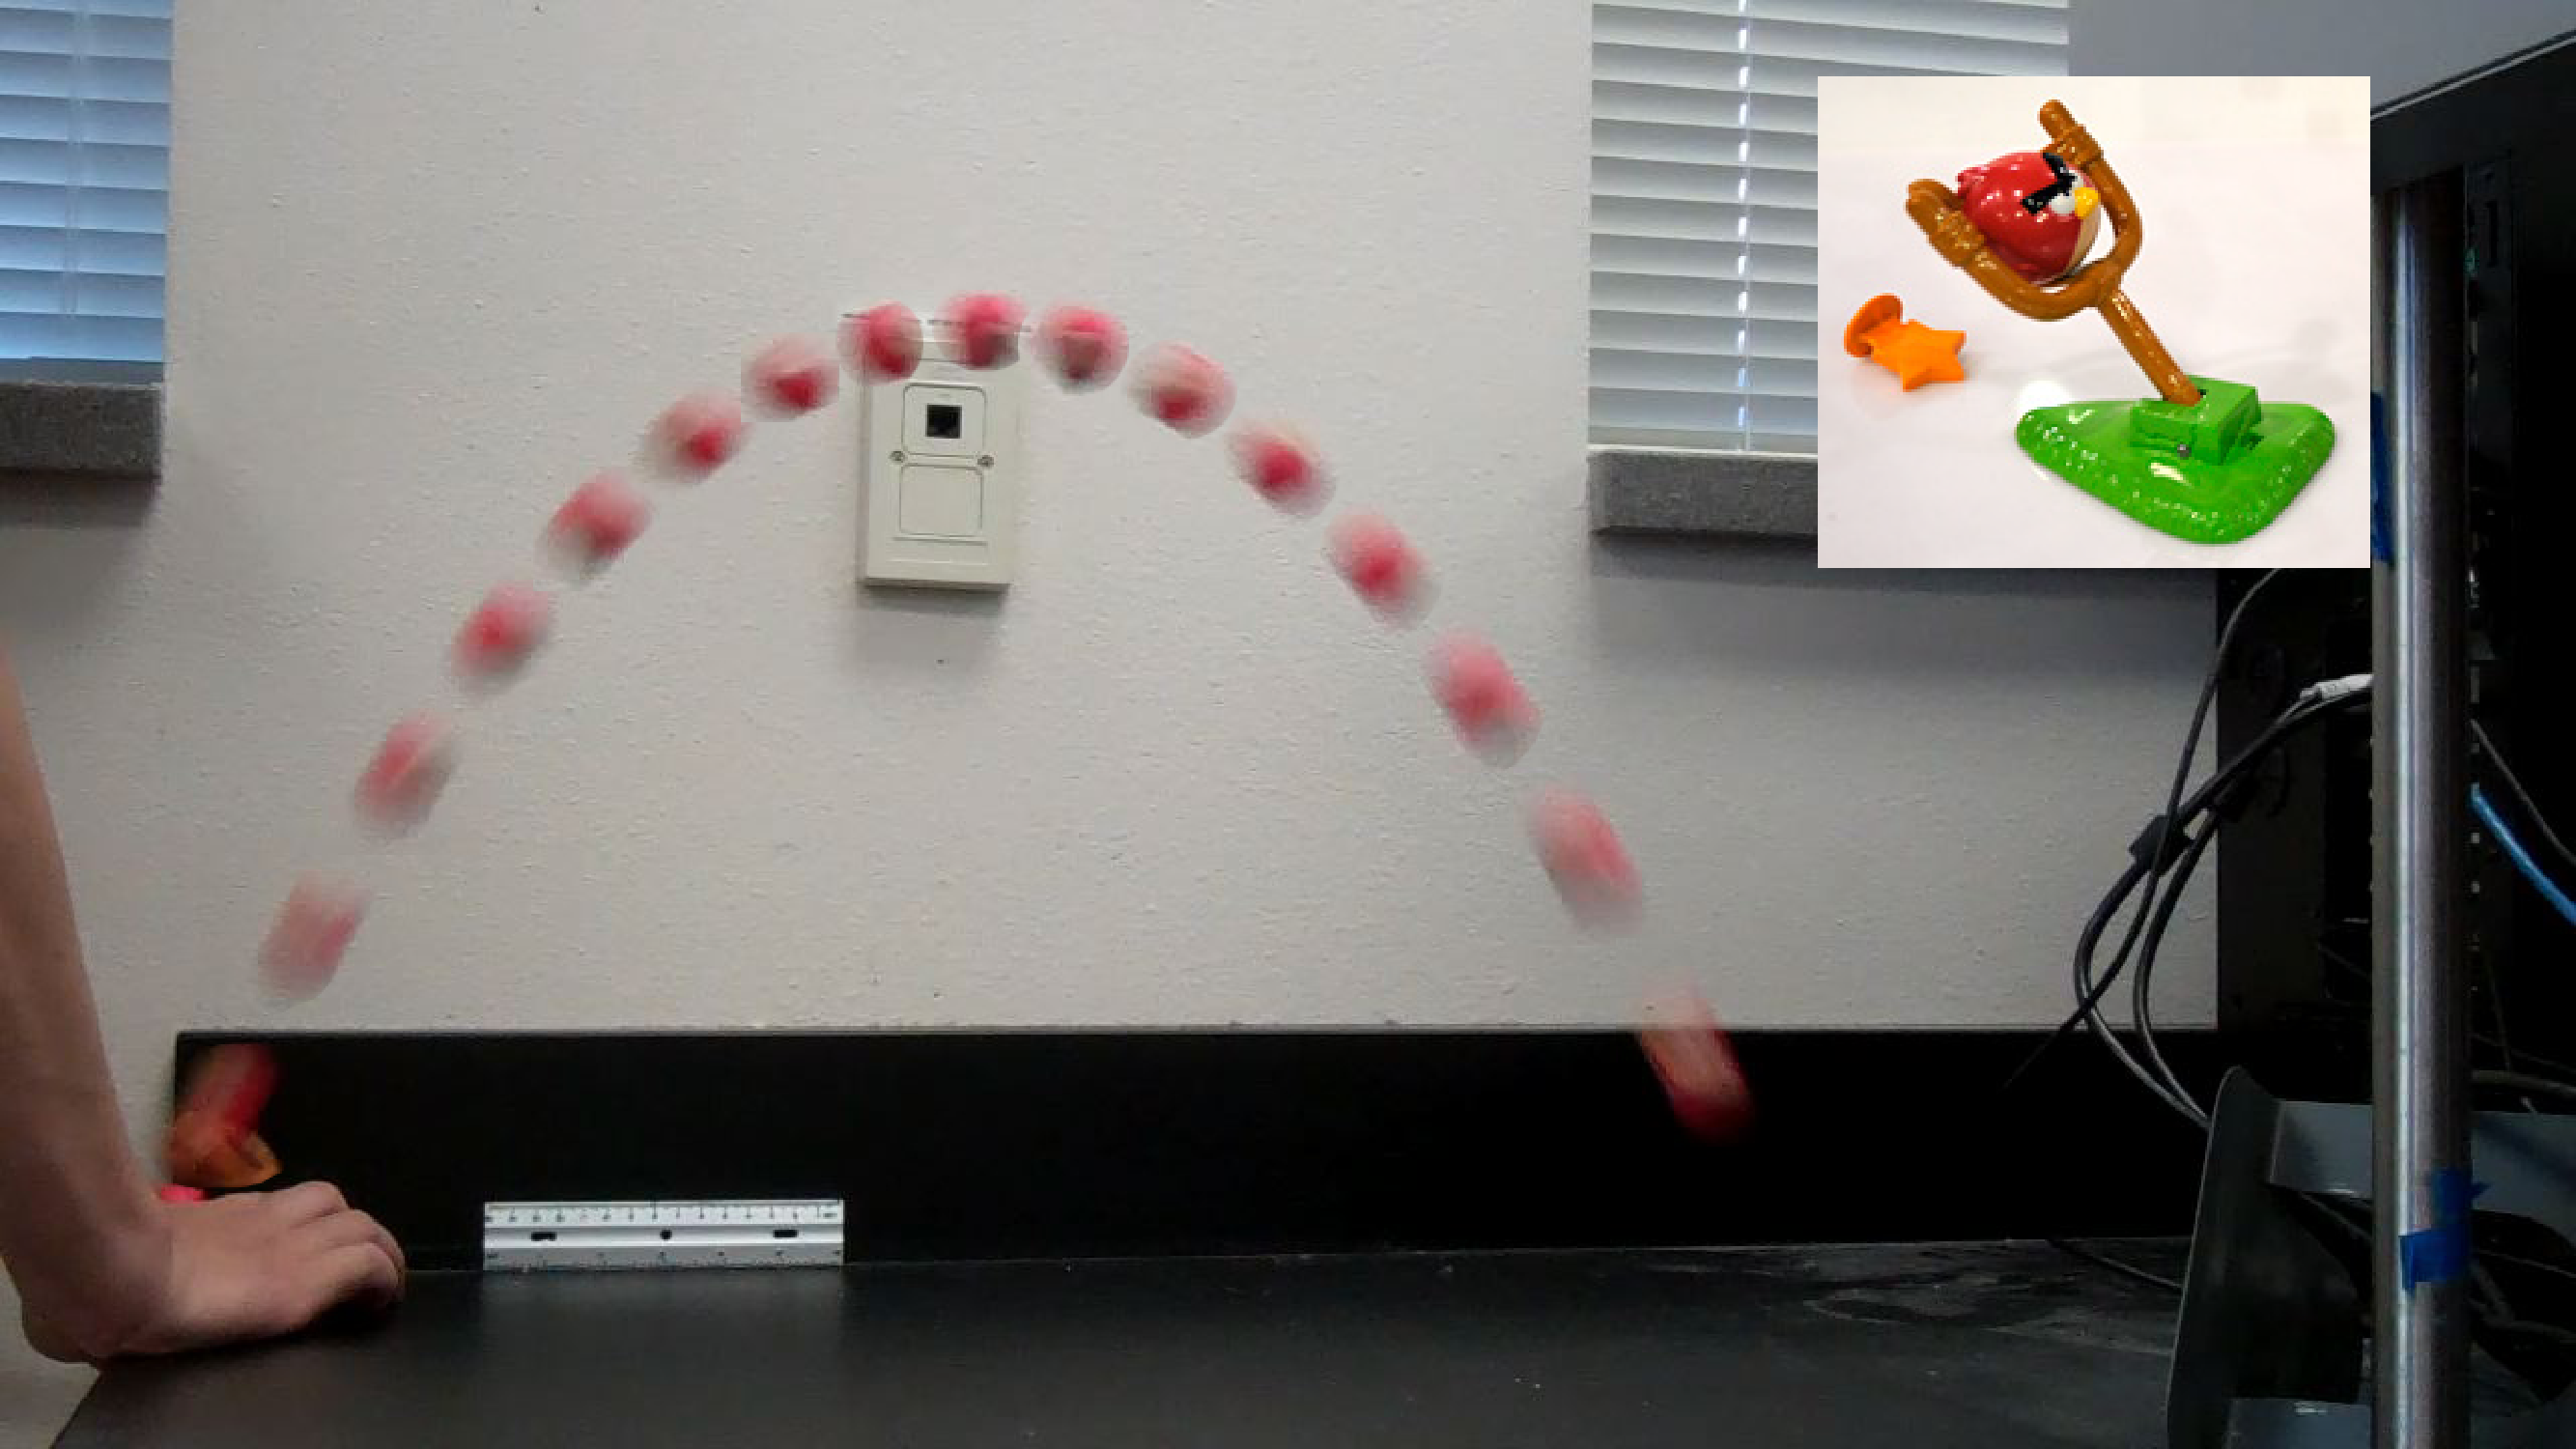
\includegraphics[width=\textwidth]{figures/tdd-AngryBirdComposite.pdf}
\caption{Trajectory of an Angry Bird.  Composite image with multiple frames superimposed, \SI{30}{frame\per\second}, elapsed time approximately \SI{0.5}{\second}. Scale \SI{15}{\centi\meter}.  Inset shows catapult device and projectile.}
\label{fig:redbird1}
\end{figure}

\begin{figure}
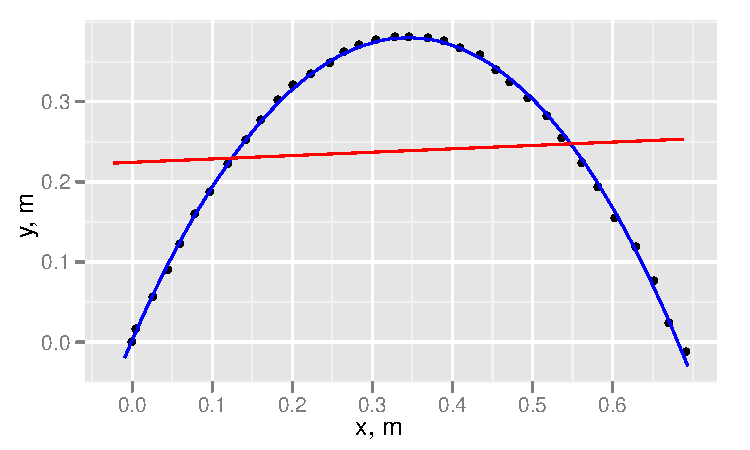
\includegraphics[width=\textwidth]{figures/tdd-angrybird2.pdf}
\caption{Digitized trajectory of an Angry Bird.  Body positions at \SI{1/60}{\second} intervals shown by dots. Blue line shows the best supported candidate models for $x(t)$ and $y(t)$.  Red line shows an unsupported candidate model.  It would be nice to add some kind of confidence interval or bootstrapping indication.}
\label{fig:redbird2}
\end{figure}

To continue with the analysis, we construct several physically-motivated candidate approximating models that we will then test to see which is best supported by the data:  

\begin{align}
\notag g_0:  x &= X_0 + \mathcal{N}(0,\sigma)& &\text{(stationary)}\\
\notag g_1:  x &= X_0 + V t + \mathcal{N}(0,\sigma)& &\text{(constant velocity)}\\
\notag g_2:  x &= X_0 + V t + \frac{1}{2}a t^2 + \mathcal{N}(0,\sigma)& &\text{(constant acceleration)}\\
\notag g_2':  x &= X_0 + V t - \frac{1}{2} \num{9.81} t^2 + \mathcal{N}(0,\sigma)& &\text{(Earth gravity)}\\
%\notag g_3:  x &= X_0 + V t + \frac{1}{2}a t^2 +\frac{1}{6}b t^3 + \mathcal{N}(0,\sigma)& &\text{(constant jerk)}\\
\notag g_3:  x &= X_0 + V t + X_1 e^{-t/\tau} + \mathcal{N}(0,\sigma)& &\text{(linear drag terminal velocity)}
\end{align}

For simplicity we consider similar forms for $y$ and assume that noise in $x$ and $y$ are uncorrelated, stationary, zero-mean Gaussian random processes $\mathcal{N}(0,\sigma)$.  Also, for a more complicated example, we might construct and solve a system of differential equations describing the motion \cite{Rauch:1965} (or see the next section). Here we work only with the trivial known forms of the solutions for simple cases. These should be adequate to describe the motion, but if they are not, we will find out from a poor fit and a large noise variance $\sigma$. 

The models were then used along with the \texttt{mle2} routine in R to obtain maximum likelihood estimates and values for the log-likelihood, AIC and BIC.  The results of the analysis are given in Tables~\ref{tbl:redbirdx} and \ref{tbl:redbirdy}. The best supported models are constant velocity ($g_1$) in $x$ and Earth gravity ($g_2'$) in $y$.  These are shown as the blue line in Figure~\ref{fig:redbird2}.  In contrast, an unsupported model, such as constant velocity ($g_1$) in $y$, shown as the red line in Figure~\ref{fig:redbird2} gives a poor fit as well as large $\Delta_i$ AIC and BIC values and low likelihood values (comparable to stationary in Table~\ref{tbl:redbirdy}).

AIC weights?

Say something about terminal velocity?  And other candidate models? mle2 seems not to be the best at finding minima without crashing into badness but we can fix that by tweaking the initial guess. Also the placement of tables 3 and 4 is somewhat problematic because of where latex wants to put the floats.  Sigh.

Compare to if we blindly took two finite differences of the raw data. Blah blah blah.   

Say something about how this can then be used to see if something is doing something other than what a passive projectile would do.  If the Angry Bird had a magic thruster that it was using to steer around a girder and come at an evil green pig from behind, we should see that by seeing that the models for passive projectiles are not supported by the altered trajectory.  

\begin{table}
\caption{Maximum likelihood parameter estimates and model comparison information for Angry Bird trajectory $x$ data of Figure~\ref{fig:redbird2}.} 
\label{tbl:redbirdx}
\begin{tabular}{lSSSSSS}
$x$ model & {$\sigma$, \SI{}{\meter}} & {$X_0$, \SI{}{\meter}} & {$V$, \SI{}{\meter\per\second}} & {$a$, \SI{}{\meter\per\second\squared}} & {$X_1$, \SI{}{\meter}} & {$\tau$, \SI{}{\second}} \\
\hline
$g_0$, stationary & \num{0.210} & \num{0.331} & \num{} & \num{} & \num{} & \num{} \\
\rowcolor[gray]{0.8} $g_1$, constant v & \num{0.007} & \num{-0.023} & \num{1.248} & & & \\
$g_2$, constant a & \num{0.005} & \num{-0.013} & \num{1.144} & \num{0.365} & & \\
$g_2'$, Earth gravity & \num{0.129} & \num{-0.279} & \num{4.031} & \num{-9.810} & & \\
$g_3$, terminal v & \num{0.010} & \num{-0.708} & \num{1.660} & \num{} & \num{0.693} & \num{1.374} \\
\end{tabular}

\begin{tabular}{lcccc}
$x$ model & $k$ & $\ln(\mathcal{L})$ & $\Delta_i\;\text{AIC}$ & $\Delta_i\;\text{BIC}$ \\
\hline
$g_0$, stationary & 2 & \num{4.93} & \num{260.2} & \num{257.1}  \\
\rowcolor[gray]{0.8} $g_1$, constant v & 3 & \num{137.03} & \num{0.0} & \num{0.0} \\
$g_2$, constant a & 4 & \num{125.75} & \num{20.6} & \num{19.0} \\
$g_2'$, Earth gravity & 3 & \num{21.98} & \num{228.1} &  \num{226.5} \\
$g_3$, terminal v & 4 & \num{-32.16} & \num{340.4} & \num{341.9} \\
\end{tabular}
\end{table}

\begin{table}
\caption{Maximum likelihood parameter estimates and model comparison information for Angry Bird trajectory $y$ data of Figure~\ref{fig:redbird2}.} 
\label{tbl:redbirdy}
\begin{tabular}{lcccccc}
$y$ model & $\sigma$, \SI{}{\meter} & $X_0$, \SI{}{\meter} & $V$, \SI{}{\meter\per\second} & $a$, \SI{}{\meter\per\second\squared} & $X_1$, \SI{}{\meter} & $\tau$, \SI{}{\second} \\
\hline
$g_0$, stationary & \num{0.126} & \num{0.238} & \num{} & \num{} & \num{} & \num{} \\
$g_1$, constant v & \num{0.127} & \num{0.224} & \num{0.052} & & & \\
$g_2$, constant a & \num{0.010} & \num{-0.036} & \num{2.877} & \num{-9.955} & & \\
\rowcolor[gray]{0.8} $g_2'$, Earth gravity & \num{0.010} & \num{-0.032} & \num{2.835} & \num{-9.810} & & \\
$g_3$, terminal v & \num{0.010} & \num{3.882} & \num{-4.647} & \num{} & \num{-3.937} & \num{0.484} \\
\end{tabular}

\begin{tabular}{lcccc}
$y$ model & $k$ & $\ln(\mathcal{L})$ & $\Delta_i\;\text{AIC}$ & $\Delta_i\;\text{BIC}$ \\
\hline
$g_0$, stationary & 2 & \num{22.56} & \num{175.4} & \num{173.9}  \\
$g_1$, constant v & 3 & \num{22.65} & \num{177.3} & \num{177.3} \\
$g_2$, constant a & 4 & \num{111.87} & \num{0.8} & \num{2.4} \\
\rowcolor[gray]{0.8} $g_2'$, Earth gravity & 3 & \num{111.28} & \num{0.0} &  \num{0.0} \\
$g_3$, terminal v & 4 & \num{-32.17} & \num{290.9} & \num{294.0} \\
\end{tabular}
\end{table}



\section{Real example:  Paper airplane}

%\section{Real example:  Amphipod, Lizard, Chukar falling}
\section{Conclusions}
It is possible to test for aerial behaviors with a minimum of statistical voodoo.  There is still some voodoo, but it is confined to a few, easy-to-understand places and one can at least rationalize the form the voodoo takes. We will now go apply what we have learned to a number of actual biological systems - amphipods, falling chukar, etc.  I might also try to use these methods on the phased array problem, and on the falling animal death curve.


\index{trajectory testing|)}


\rcsid{$Id$}
\rcsid{$Header$}
\rcskwsave{$Author$}
\rcskwsave{$Date$} 
\rcskwsave{$Revision$}

\chapter{Modeling multi-axis zero angular momentum turns}
\label{app:ang}
\index{inertial method|(}
These notes give my thoughts on how to numerically test a recorded movement for use of zero- and constant angular momentum turning mechanics\footnote{Tom Daniel first suggested to me the idea of predicting what an animal would do if there were no air, in the solely inertial case.}.

\section{Introduction}
We wish to examine the earliest instants of roll, pitch, and yaw maneuvers made by baby birds (Chukar Partridge (\emph{Alectoris chukar}) and Mallard Duck (\emph{Anas platyrhynchos}), from \SI{1}{dph} to fledging).  At this early age, the wings are not yet fully developed.  In addition, during the initial instants of a fall, the body has not yet attained sufficient airspeed to develop large aerodynamic forces and torques, which scale $\sim \rho U^2 A$ and $\rho U^2 A \lambda$, respectively.  Consequently we might expect these early maneuvers to involve significant contribution from other mechanisms, such as inertial mechanisms \cite{Edwards:1986, Jusufi:2008, Jusufi:2010}.  Inertial mechanisms are ones in which body angular position is changed by modulating body inertia, either to modulate some initial angular momentum obtained when leaving the ground, or to effect a zero- or constant angular momentum turn \cite{Edwards:1986}.  In order to answer questions of biological interest, we need general ways (numerical methods) to test if a given maneuver uses inertial mechanisms or detect when non-inertial mechanisms must be at work. 






\subsection{Conservation of angular momentum $H$}
First, some definitions are in order.  For a collection of moving particles, we can define angular momentum about an arbitrary point $B$ as follows (after \cite{Baruh:1999}):
\begin{equation}
\vec{H}_B = \sum_i \vec{r}_{Bi} \times m_i \vec{v}_i
\end{equation}
We also introduce the centroid, or center of mass $G$: 
\begin{equation}
\vec{r}_G = \frac{\sum_i m_i \vec{r}_i}{\sum_i m_i}
\label{eq:COM}
\end{equation}
which, for our collection of moving particles, may also be moving.  The angular momentum about the center of mass reduces to a convenient form:
\begin{equation}
\frac{d}{dt} \vec{H}_G = \vec{M}_G
\end{equation}
where $M_G$ are the externally applied moments about the center of mass. In the case of an organism in free fall, where it has not yet attained sufficient speed for aerodynamic torques to be significant, and is not ejecting any mass or in contact with things that it can push off on (refer to \cite{Baruh:1999} for the derivation of this result) 
\begin{equation}
\frac{d}{dt} \vec{H}_G = 0
\end{equation}
or alternatively,
\begin{equation}
\vec{H}_G = \sum_i \vec{r}_{Gi} \times m_i \vec{v}_i = \mbox{constant}
\label{eq:zam}
\end{equation}
In other words, angular momentum is conserved.  

Equation~\ref{eq:zam} will be the main tool we use in our simulations and analyses in two ways.  First, we will take observations of body position and calculate $H_G$, to test if angular momentum is constant and detect if a maneuver requires use of external (aerodynamic) torques. This first task is easy.  Second, given a sequence of body positions in coordinates fixed to the body, we should be able to project what whole-body rotations should result in the absence of air, i.e.\ if the animal were magically flying in a vacuum.  The second task is only a little harder. 






\subsection{Calculating $H$ from observed positions, the easy way}
\label{sec:forward}
By filming an organism with multiple calibrated cameras, it is often possible to obtain estimates of three-dimensional position for joints, markers, limbs, etc.  We denote these measured positions as a set of position vectors in the rest frame $\vec{r}_{0i}[n]$, where $[n]$ represents each discrete time frame of the video.  

With each point we will also associate a point mass $m_i$ representing the mass of each chunk of the organism. This is a simplification; organisms are not point masses in general, but small chunks of an animal can be approximated as such to simplify calculation\footnote{We really really really wish to avoid dealing with long kinematic chains where each link has large inertia; any more than two links is very hard to write and likely to induce madness.}. We can guess $m_i$ from the shape of the animal, or by using a good balance and a meat cleaver. Unless chunks of the organism are removed or redistributed during the sequence (not usually the case for terrestrial animals), $m$ does not depend on time $[n]$. Thus, our analysis model of the organism is a system of point masses with prescribed motions.  

To numerically calculate the angular momentum $H$ of the system, we proceed by finding the location of the center of mass $\vec{r}_G$ using Equation~\ref{eq:COM} above. We subtract to find the time-varying body positions relative to the time-varying center of mass:
\begin{equation}
\vec{r}_{Gi}[n] = \vec{r}_{0i}[n]-\vec{r}_{G}[n]
\label{eq:rg}
\end{equation}
The velocity of each point mass, $\vec{v}_{Gi}[n]$, can be estimated using a simple backwards difference:
\begin{equation}
\vec{v}_{Gi}[n] \approx \frac{\vec{r}_{Gi}[n] - \vec{r}_{Gi}[n-1]}{\Delta t}
\end{equation}
where $\Delta t = 1/\mbox{fps}$ is the period between frames. Taking derivatives of positional data injects noise, but this is the only derivative we need to take, and hopefully it's not as bad as differentiating twice to get accelerations\footnote{If this does turn out to be bad, there are other tricks we can try like spline smoothing or using more explicit models of the body. This is one of those we'll cross our fingers and hope it's OK situations.}. 

We now have all the pieces needed to compute $H_G$ at each time step $[n]$, repeated here: 
\begin{equation}
\vec{H}_{Gi}[n] = \vec{r}_{Gi}[n] \times m_i \vec{v}_{Gi}[n]
\end{equation}
\begin{equation}
\vec{H}_{G}[n] = \sum_i \vec{H}_{Gi}[n]
\end{equation}

For a zero- or constant angular momentum (inertial) maneuver, $H_G[n]$ should be constant, while for a maneuver where external aerodynamic torques are important, $H_G[n]$ will vary with time. Plotting should suffice to tell, or this could be formally tested using maximum likelihood estimation plus an Akaike Information Criterion \cite{notes:tdd}. 

The principal advantage of this numerical formulation is that it is easier to apply to more generalized shapes (e.g.\ a baby bird with two kicking legs, two flapping wings, wagging tail and a head on a long neck; insect with six legs) compared to analytical models of chains of inertias that must be specifically derived for each body plan \cite{Jusufi:2008, Jusufi:2010, Evangelista:unpub2} and which are usually only tractable for small numbers of links.  Kinematics studies naturally produce positions of points, which can easily be used to generate clouds of point masses that track the movements of the study organism and allow computation of its angular momentum. 






\subsection{Predicting body rotation to maintain $H$ constant}
\label{sec:reverse}
We may wish to go the ``opposite'' way in our numerical analysis, in other words, find the expected motions if the maneuver was only inertial.  In this case what we do is a little different.  We begin as before, with a set of position vectors $\vec{r}_{0i}[n]$ for each joint/marker/limb/point as it moves through time $[n]$. We also assume or measure the mass associated with each chunk $m_i$, and we compute the time-varying position of the center of mass $\vec{r}_G$ (Equation~\ref{eq:COM}). From this we use Equation~\ref{eq:rg} to obtain $\vec{r}_{Gi}[n]$, the time-varying body positions relative to the center of mass. So far this is the same as in Section~\ref{sec:forward}. 

In Section~\ref{sec:forward}, we computed $\vec{r}_{Gi}[n]$ in a reference frame that is translating with the center of mass but is not rotating.  Consider instead a reference frame$'$ that translates with the center of mass and also rotates with some logical body-fixed axes, such as in an anatomically bilaterally symmetric animal (antero-posterior, lateral, and dorso-ventral axes)\footnote{It need not be strictly bilaterally symmetric in the posture taken during the maneuver.}.  We denote the body position in the new frame$'$ as:
\begin{equation}
\vec{r}'_{Gi}[n] = \mathbf{R}[n] \cdot \vec{r}_{Gi}[n]
\label{eq:rotation}
%\label{eq:start-reverse}
\end{equation}
where $\mathbf{R}[n]$ is an appropriately chosen, invertible rotation matrix. With the body positions in the new coordinate system, we continue as before to obtain the velocities and ``apparent'' angular momentum:
\begin{equation}
\vec{v}'_{Gi}[n] \approx \frac{\vec{r}'_{Gi}[n] - \vec{r}'_{Gi}[n-1]}{\Delta t}
\end{equation}
\begin{equation}
\vec{H}'_{Gi}[n] = \vec{r}'_{Gi}[n] \times m_i \vec{v}'_{Gi}[n]
\label{eq:fakeH}
\end{equation}
\begin{equation}
\vec{H}'_{G}[n] = \sum_i \vec{H}'_{Gi}[n]
\label{eq:apparent}
\end{equation}
For an inertial maneuver, $H'_G[n]$ will usually \emph{not} be constant because we removed the whole-body rotation when we transformed to a coordinate frame that rotates with the body. Using this discrepancy, we can find the whole-body rotation that would have made the ``real'' angular momentum $H_G$ constant. 

Recall that the ``real'' angular momentum for the case of no external torques $H_{Gi}[n]$ is given by
\begin{equation}
\vec{H}_{G}[n] = \sum_i \vec{r}_{Gi}[n] \times m_i \vec{v}_{Gi}[n] = \mbox{constant} = \vec{H}_G[0]
\end{equation}
Since $\mathbf{R}$ is invertible\footnote{In the case of a body with zero initial angular momentum ($\vec{H}_G[0] = 0$) we can avoid calculating $\mathbf{R}$ entirely! Win!}, we can expand using Equation~\ref{eq:rotation}, keeping in mind that the velocities of each mass also include a component from the whole-body rotation:
\begin{equation}
\vec{H}_{G}[n] = \sum_i \mathbf{R}^{-1}[n] \cdot \vec{r}'_{Gi}[n] \times m_i (\vec{v}'_{Gi}[n] + \vec\omega_G[n] \times \vec{r}'_{Gi}[n] ) = \vec{H}_G[0]
\end{equation}
We then rearrange terms and simplify: 
\begin{equation}
\sum_i \vec{r}'_{Gi}[n] \times m_i (\vec{v}'_{Gi}[n] + \vec\omega_G[n] \times \vec{r}'_{Gi}[n]) = 
\mathbf{R}[n] \cdot \vec{H}_G[0] 
\end{equation}
\begin{equation}
\sum_i \vec{r}'_{Gi}[n] \times m_i \vec{v}'_{G,i}[n] + 
\sum_i \vec{r}'_{Gi}[n] \times m_i \vec\omega_G[n] \times \vec{r}'_{Gi}[n] = 
\mathbf{R}[n] \cdot \vec{H}_G[0] 
\end{equation}
\begin{equation}
\vec{H}'_G[n] +
\mathbf{J}'_G[n] \vec\omega_G[n] = \mathbf{R}[n] \cdot \vec{H}_G[0] 
\end{equation}
\begin{equation}
\vec\omega_G[n] = 
\mathbf{J}_G^{\prime -1}[n] \cdot (\mathbf{R}[n] \cdot \vec{H}_G[0]
-\vec{H}'_G[n]) 
\label{eq:end-reverse}
\end{equation}
where $\mathbf{J}'_G[n]$ are the instantaneous moments of inertia of the body about the body-fixed ($'$) axes and $\vec\omega_G[n]$ is the whole-body rotational speed. It is worthwhile to write out $\mathbf{J}'_G[n]$ and equation~\ref{eq:end-reverse} for the case of zero initial angular momentum ($\vec{H}_G[0]=0$). 
\begin{equation}
\vec\omega_G[n] = 
- \mathbf{J}_G^{\prime -1}[n] \cdot 
\vec{H}'_G[n] 
\label{eq:end-reverse1}
\end{equation}
\begin{equation}
\mathbf{J}'_G[n] = 
\sum_i \begin{bmatrix}
m_i (r_{iy}^2+r_{iz}^2) & -m_i r_{ix} r_{iy} & -m_i r_{ix} r_{iz} \\
-m_i r_{ix} r_{iy} & m_i (r_{ix}^2+r_{iz}^2) & -m_i r_{iy} r_{iz} \\
-m_i r_{ix} r_{iz} & -m_i r_{iy} r_{iz} & m_i (r_{ix}^2+r_{iy}^2) 
\end{bmatrix}
\label{eq:Jn}
\end{equation}
where all $\vec{r}_i$ are evaluated at time $[n]$.  

Using equations~\ref{eq:end-reverse1}, \ref{eq:Jn}, and \ref{eq:apparent}, we can numerically integrate $\vec\omega_G[n]$ to find $\vec\theta_G[n]$, the angular position of the body, and then construct a new rotation matrix $\mathbf{A}[n]$ to rotate the entire body to the new predicted orientation.  We also translate the center of mass according to which external conservative forces (e.g.\ gravity) are acting.

Equations~\ref{eq:end-reverse1}, \ref{eq:Jn}, and \ref{eq:apparent} allow us to predict the overall motion of a body given prescribed appendage movements (flapping, kicking, tail wagging) with respect to body-fixed coordinates.  To be sure the numerical methods work correctly, we can check these methods and those from Section~\ref{sec:forward} using simple toy model simulations (Section~\ref{sec:toy}) and actual measured data (Section~\ref{sec:real}). 

\section{Simulation of a two-dimensional toy model}
\label{sec:toy}

\begin{figure}
%A \includegraphics[width=0.4\textwidth]{figures/untitled.jpg}
%B \includegraphics[width=0.4\textwidth]{figures/zam-fling.jpg} \\
%C \includegraphics[width=0.4\textwidth]{figures/nonzam-fling.jpg}
%D \includegraphics[width=0.4\textwidth]{figures/zam-joint-pos.jpg}

\caption{A. Tumbling amphipod with constant length body showing constant total angular momentum. B. Tumbling amphipod with body shortening at time $t=0.4$, showing rotational speed up to maintain constant total angular momentum. C. Tumbling amphipod with rocket motors firing at time $t=0.4$ and retro-rockets at $t=0.6$, showing non-constant total angular momentum. D. Two-link ``gecko'' with lateral tail wagging \ang{\pm 30} at \SI{3}{\hertz} in body-fixed coordinates (left) and with projected motion assuming zero total angular momentum (right).}
\label{fig:toysim}
\end{figure}

%\subsection{Constant angular momentum case}
%\subsection{Non-constant angular momentum case}
%\subsection{Inertial yawing of a two-link ``gecko''}

%This is an example of a table:
%\begin{table}
%\caption{Hello world in table form.}
%\label{tab:hello}
%\begin{tabular}{lr}
%Able & Baker \\
%Charle & Dog \\
%\end{tabular}
%\end{table}

%\section{Results from actual measured kinematics}
%\label{sec:real}

%\subsection{Real amphipod pitch in yaw, 2-D}
%\subsection{Gecko roll from Full lab}
%\subsection{Hummingbird yaw maneuver - should be nonZAM} 
%\subsection{Diver or skydiver pitching and rolling?}


%\section{Conclusions}

% AMS style references
%\bibliographystyle{amsplain}
%\bibliography{references/modeling-turns}
\index{inertial method|)}



\pagestyle{plain}
\bibliography{references/thesis}
\printindex

\end{document}
